\documentclass[11pt,a4paper]{article}
%
% PACKAGES
\usepackage[margin=2cm]{geometry}
\usepackage{setspace}
\usepackage{graphicx}
\usepackage{amsmath}
\usepackage{siunitx}
\usepackage{booktabs}
\usepackage{caption}
\usepackage{hyperref}
\usepackage{nomencl}
\usepackage{tocloft}
\usepackage{tabularx}
\usepackage{float}
\usepackage{etoolbox}
\usepackage{pgfgantt}
\usepackage{array}
\usepackage{cleveref}
\usepackage{tikz}
\usepackage{pdflscape}
\usetikzlibrary{positioning, arrows.meta}

\newcommand{\secref}[1]{[\ref{#1}]}
%nomenclature
\renewcommand{\nomgroup}[1]{%
  \item[\bfseries
  \ifstrequal{#1}{A}{Symbols}{%
  \ifstrequal{#1}{B}{Greek Symbols}{}}%
]}
\makenomenclature

%flowchart
\usepackage{tikz}
\usetikzlibrary{shapes.geometric, arrows.meta, positioning}
\tikzstyle{startstop} = [rectangle, rounded corners, minimum width=3cm, minimum height=1cm,text centered, draw=black]
\tikzstyle{process} = [rectangle, minimum width=3cm, minimum height=1cm, text centered, draw=black]
\tikzstyle{decision} = [diamond, minimum width=3cm, minimum height=1cm, text centered, draw=black]
\tikzstyle{arrow} = [thick,->,>=Stealth]

\setstretch{1.5}
%------------------------------------------------
\begin{document}

%--------------------------------------------------------
% TITLE PAGE
\begin{titlepage}

\centering

\vspace{1cm}

{\Huge \textbf{Design Report}}

\vspace{1cm}

{\Large Design of a Portable Hybrid Renewable Energy System for an Arctic Exploration Camp }
\vspace{0.5cm}

\textbf{Project ID}\\
MBPW2

\vspace{0.5cm}

\textbf{Authors}

Cameron Jones \quad Ibrahim Kamran \quad Nicholas Wright \\ Oliver Montorio \quad Samuel Olliffe \quad Timothee Breabout

\vspace{1cm}

\textbf{Supervisors}

Peter Waugh \quad Majid Bastankhah

\vspace{1cm}

\textbf{Date}

\today

\vspace{1cm}


\begin{figure}[H]
    \centering
    \includegraphics[width=0.8\textwidth]{figures/Design_Image.png}
    \caption{Final Assembly Design }
    \label{fig:FinalDesign}
\end{figure}

\vfill

\end{titlepage}

%--------------------------------------------------------
% EXECUTIVE SUMMARY
\begin{center}
    {\LARGE \textbf{Executive Summary - SO}} \\[4pt]
    {\normalsize EastGRIP Remote Research Camp, North-East Greenland}
\end{center}

\vspace{2pt}

This project aimed to design and develop a deployable device capable of generating sustainable electrical energy while simultaneously recording key environmental data to assess the feasibility of renewable power generation at the EastGRIP remote research camp in north-east Greenland --- a site that operates exclusively between April and August. The device is intended to reduce the camp's dependence on diesel generators, lower operational fuel costs, and provide a quantitative basis for evaluating renewable energy potential in high-latitude, arctic environments.

The principal engineering challenges were twofold: achieving consistent and meaningful power output under variable arctic conditions, and ensuring the reliable operation of all mechanical and electronic components across the full range of expected environmental extremes. Operating conditions at EastGRIP can reach \(-30\,^{\circ}\mathrm{C}\) with wind speeds up to 40\,kt, imposing severe constraints on material selection, thermal management, and structural integrity.

The proposed system integrates a horizontal-axis wind turbine with six bifacial solar panels, both mounted on a purpose-engineered structural base that also houses the battery bank and electrical circuitry. The mast, which extends 2.5\,m vertically, is stabilised by four guy ropes, while the base is secured to the ice surface via drilled anchor plates, providing resistance to wind loading.

Environmental and performance data are collected through a suite of sensors: a pyranometer, an anemometer, two temperature sensors, and individual power sensors monitoring the output of both the solar array and the wind turbine. All sensor data is processed by a central microcontroller and logged on a removable SD card, enabling periodic physical retrieval by camp personnel.
Thermal management is addressed by a PTC-regulated internal heater within the electrical enclosure, maintaining a minimum internal temperature of \(0\,^{\circ}\mathrm{C}\). The PTC element self-limits power draw once the target temperature is reached, preventing unnecessary energy consumption.

The system is projected to generate approximately \textbf{2{,}850\,kWh} over the five-month operational period, with solar panels accounting for an estimated 91\% of total output and the wind turbine contributing the remaining 9\%. This distribution reflects the near-continuous solar irradiance characteristic of the arctic summer at this latitude.
While this output is insufficient to fully displace diesel generation at the camp, it represents a substantial reduction in fossil fuel consumption. The total system cost is estimated at \textbf{£9{,}209}, with projected fuel savings expected to recover the capital expenditure within approximately one to two years.
Although all performance estimates are calibrated to the EastGRIP site, the system architecture is transferable to other arctic and sub-arctic deployments. It should be noted that solar output may be reduced at sites with lower solar irradiance, and wind turbine performance may be affected by terrain-induced flow interference. These factors should be assessed on a site-specific basis for any future deployment.

\newpage

%--------------------------------------------------
% CONTENTS
%--------------------------------------------------
\tableofcontents
\newpage

\listoffigures
\newpage

\listoftables
\newpage

\section{}
% NOMENCLATURE

\nomenclature[A]{$V$}{Voltage (V)}
\nomenclature[A]{$I$}{Current (A)}
\nomenclature[B]{$\eta$}{Efficiency (\%)}
\nomenclature[A]{$E$}{Energy (J)}
\nomenclature[A]{$A_{Surface}$}{Base Surface Area}
\nomenclature[A]{$Q$}{Heat Transfer}
\nomenclature[A]{$k$}{Thermal Conductivity}
\nomenclature[B]{$\Delta T$}{External to Internal Temperature Difference}
\nomenclature[A]{$L$}{Wall Thickness}
\nomenclature[A]{$l$}{Characteristic Base Length}
\nomenclature[A]{$w$}{Characteristic Base Width}
\nomenclature[A]{$h$}{Characteristic Base Height}
\nomenclature[A]{$T_{inside}$}{Internal Temperature of Base}
\nomenclature[A]{$T_{outside}$}{External Temperature Outside Base}
\nomenclature[A]{$W$}{Watts}
\nomenclature[A]{R}{Thermal Resistance}
% Nomenclature entries for wind-energy bin model
\nomenclature[A]{$E_T$}{Expected energy over period $T$ [kWh]}
\nomenclature[A]{$E_i$}{Energy from wind-speed bin $i$ over period $T$ [kWh]}
\nomenclature[A]{$T$}{Evaluation period duration [h]}
\nomenclature[B]{$N$}{Number of wind-speed bins [--]}
\nomenclature[B]{$i$}{Wind-speed bin index, $i=1,\dots,N$ [--]}
\nomenclature[A]{$v$}{Wind speed [m s$^{-1}$]}
\nomenclature[A]{$v_{i-1},\,v_i$}{Lower/upper edges of wind-speed bin $i$ [m s$^{-1}$]}
\nomenclature[A]{$v_i^{\ast}$}{Representative speed for bin $i$ (midpoint) [m s$^{-1}$]}
\nomenclature[A]{$P(v)$}{Turbine electrical power at wind speed $v$ [W]}
\nomenclature[A]{$P(v_i^{\ast})$}{Power at $v_i^{\ast}$ from digitised curve [W]}
\nomenclature[B]{$F_V(v)$}{CDF of wind speed, $\mathbb{P}(V\le v)$ [--]}
\nomenclature[B]{$p_i$}{Bin probability, $F_V(v_i)-F_V(v_{i-1})$ [--]}
\nomenclature[A]{$V$}{Wind-speed random variable (units as $v$)}
%nomclature for guy ropes and groundings
\nomenclature[A]{$F$}{Force [N]}
\nomenclature[B]{$\rho$}{Air density [kg m$^{-3}$]}
\nomenclature[A]{$C_d$}{Drag coefficient}
\nomenclature[A]{$M$}{Moment (Nm)}

%SOLAR + APPENDIX A%
\nomenclature[B]{$\theta $}{Tilt angle (^\circ)}
\nomenclature[B]{$\phi $}{Nominal tilt (^\circ)}
\nomenclature[B]{$\phi_{season} $}{Seasonal adjustment (^\circ)}

\nomenclature[A]{$E_{solar} $}{Solar energy (kWh)}
\nomenclature[A]{$H_{ip} $}{In-plane irradiation (kWh/m$^{2}$)}
\nomenclature[A]{$A_{total} $}{Total area of the panels (m$^{2}$)}
\nomenclature[B]{$\eta_{panel}  $}{Panel rated efficiency (\%)}
\nomenclature[A]{$PR $}{Performance ratio of panels }

\nomenclature[B]{$\phi_{\text{adj}}$}{Adjustment tilt (^\circ)}

%APPENDIX B%

\nomenclature[A]{$A_{\text{proj}}$}{Projected panel area (m$^{2}$)}
\nomenclature[A]{$A_{\text{panel}}$}{Panel area (m$^{2}$)}
\nomenclature[A]{$F_L$}{Lift force (N)}
\nomenclature[A]{$F_{L,\text{net}}$}{Net lift force (N)}
\nomenclature[A]{$W_{\text{panel}}$}{Weight of a panel (N)}
\nomenclature[A]{$W_{\text{mount}}$}{Weight of a mount (N)}
\nomenclature[B]{$\tau_{\text{ice}}$}{Shear resistance of ice (Pa)}
\nomenclature[A]{$F_D$}{Drag force (N)}
\nomenclature[A]{$n_{\text{total}}$}{Total number of supports per mount }
\nomenclature[A]{$n_{\text{front}}$}{Number of front supports per mount }




\printnomenclature
\newpage

%===============================================
% MAIN REPORT
%===============================================
\section{Introduction}

\subsection{Problem definition - CJ}
Reliable energy generation remains a major challenge for remote Arctic research stations, where logistical constraints and extreme environmental conditions severely limit conventional power infrastructure. The objective of this project is to design a deployable device capable of generating renewable energy using multiple production methods while simultaneously collecting data to evaluate the feasibility of sustainable energy generation in Arctic environments.

The selected deployment site is the East Greenland Ice-core Project (EastGRIP) camp, located within Northeast Greenland National Park inside the Arctic Circle. The site provides extensive environmental monitoring data, enabling accurate assessment of local conditions to inform engineering design decisions. EastGRIP is highly isolated, located approximately 350 km from the nearest ice-sheet research station and around 690 km from the nearest settlement, Ittoqqortoormiit, making conventional energy supply difficult.

Most polar research stations rely on diesel generators, which require regular fuel transport and introduce significant logistical cost and environmental risk. However, the exposed ice-sheet location of EastGRIP at an altitude of approximately 2700 m provides favourable conditions for renewable energy generation. High wind speeds and prolonged Arctic daylight during the station’s operational season (April–August) create opportunities for a hybrid wind–solar system.

Deployment logistics further constrain the design, as all equipment must be transported via LC-130 Hercules aircraft, requiring a modular and lightweight system compatible with aircraft pallet dimensions and payload limits.

\subsection{Stakeholders - CJ}
A stakeholder analysis was conducted to identify organisations with significant influence over the project. Two primary key stakeholders were identified: the East Greenland Ice-core Project (EastGRIP) camp and the Centre for Ice and Climate at the University of Copenhagen. As the University of Copenhagen currently provides financial support for the EastGRIP research programme, it is expected that this organisation would also act as the primary funding body for the proposed system. Consequently, the Centre for Ice and Climate has been treated as the principal stakeholder, and the design has been developed with particular consideration for its research objectives, operational requirements, and long-term sustainability goals.

\begin{table}[H]
\centering
\caption{Stakeholder analysis for the EastGRIP renewable energy system.}
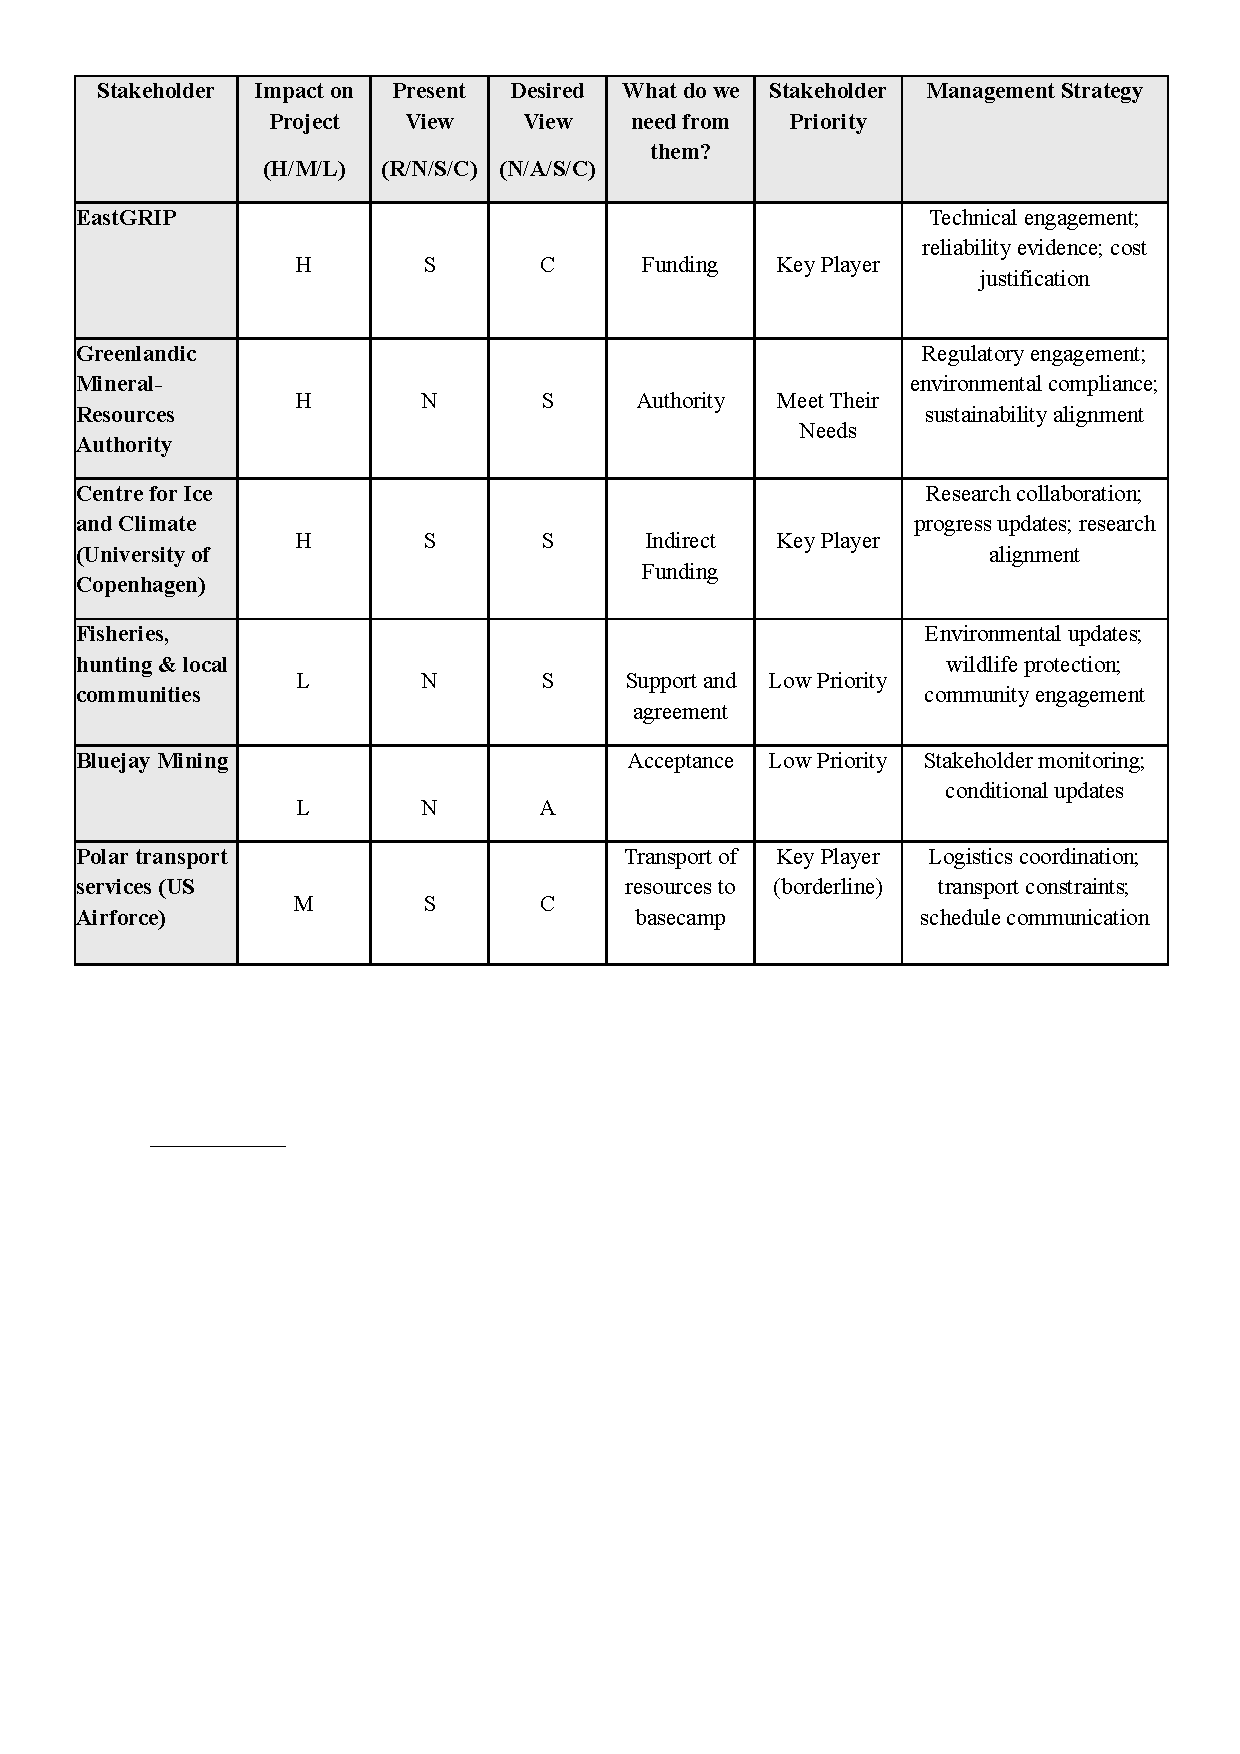
\includegraphics[width=\textwidth, trim=0 13cm 0 1cm, clip]{tables/StakeHolders.pdf}
\end{table}

{\footnotesize
\textbf{Notes:} \quad H = High, M = Medium, L = Low.

R = Resistant, N = Neutral, S = Supportive, C = Committed, A = Accept.

KP = Key Player, MTN = Meet Their Needs, KI = Keep Informed, LP = Low Priority.
}

\subsection{Design Specifications \& Existing Solutions - TB}

Thoughtout the design process, the system is guided by the User Requirements Specification (URS) that was developed during the feasibility study. These requirements accentuate the key technical constraints that the device must satisfy so that it can operate reliably at the EastGRIP research camp. These specifications primarily address the logistical constraints such as transportability and the packed dimensions, environmental conditions which include low temperatures and high wind speeds, but also functional targets such as power production and system cost.

The Table ~\ref{tab:URS} summarises all the main requirements that have guided the development of the system design. These criteria were used throughout the detailed design process as a way to ensure that the final product stays compatible with the operational, environmental, and economic constraints of the project.

\begin{table}[H]
  \centering
  \caption{Summary of User Requirements Specification}
  \label{tab:URS}
  \begin{tabular}{llp{7cm}l}
    \toprule
    Code & Spec & Quantity / Description & Source \\ \midrule
    M1 & Weight & Total system mass $< \SI{3}{t}$ & \cite{Weight} \\
    M2 & Unpacked dimension & Maximum operating height $< \SI{4}{m}$ & \cite{Power Production} \\
    M3 & Packed dimension & Must fit on aircraft pallet
          (\SI{2.64}{m} $\times$ \SI{2.13}{m} $\times$ \SI{2.40}{m}) & \cite{Packed Dimensions} \\
    M4 & Power production & Offset $\approx 1~\%$ of \SI{0.17}{MWh/day}
         ($\approx\SI{1.7}{kWh/day}$) & \cite{Power Production} \\
    M5 & Wind resistance & Safe operation up to \SI{40}{kt} wind speed & \cite{Weather} \\
    M6 & Temperature constraint & No damage at \(-\SI{30}{\celsius}\) & \cite{Weather} \\
    M7 & Internal heating & Maintain battery temperature at \SI{0}{\celsius} & \cite{Internal Heating} \\
    M8 & Battery/circuit insulation & Thermal insulation sufficient to
         hold \SI{0}{\celsius} with minimal heating power & \cite{Battery Final} \\
    M9 & Ice resistance & Turbine de-icing to clear \SIrange{4}{7}{mm}
         ice accretion & \cite{Weather} \\
    M10 & Cost & Total cost $\leq$ cost of \(1~\%\) of seasonal fuel use across lifetime [15 years]
           ($\approx 15\% \text{ of } \$57{,}000$
)& \cite{Fuel Price} \cite{Fuel usage} \\
    W1 & Sensor data accessibility & System data updated at least every 30~min & \\
    W2 & Wind-speed sensor & Wind speed recorded every 30~min &  \\
    W3 & Ice-weight measurement & Ice mass measured daily &  \\
    W4 & Solar measurement & Solar irradiance / PV power logged every 10~min & \\
    \bottomrule
  \end{tabular}
\end{table}

\subsection{Report Structure - CJ}
The remainder of this report describes the development of the proposed system. Section 2 presents the design concept and system architecture, followed by detailed design considerations. Manufacturing, sustainability, and commercial factors are then evaluated before the final design is assessed against alternative solutions.


%--------------------------------------------------
\section{Design Development - TB}
\subsection{Initial Concept}
The first design concept required the ability to provide renewable energy generation through the use of locally available environmental resources. An in-depth analysis of meteorological data for the EastGRIP region provided sufficient information to conclude that the site would experience strong and consistent wind conditions and a near-continuous solar exposure during the summer months. This information validated the theory that a hybrid wind-solar system would provide the most reliable energy generation on site.

From the first concept, three major subsystems were identified:
\begin{itemize}
\item A small-scale wind turbine attached to a deployable mast
\item An array of photovoltaic solar panels
\item A logging system that enables the collection and storage of environmental sensing and data 
\end{itemize}

The energy produced by renewable sources is stored within a battery system, all the while enabling the sensors and data logging system to operate continuously even in the event of short periods of reduced generation.

This hybrid architecture was chosen to reduce the reliability risks that occur when using a single renewable source. For example, during storms or heavy cloud cover, solar power generation can be drastically reduced. On the other hand, wind generation can vary significantly depending on local wind conditions. Therefore, combining the two systems allows the design to maintain a more stable power supply and guarantee the full functionality of the concept under varying environmental conditions and locations.

\subsection{Concept Evaluation}
As a continuation of the feasibility stage, the design process focused mainly on refining and improving the previously selected system architecture rather than redefining the overall concept. The feasibility report had already confirmed the use of a telescopic mast and a small-scale wind turbine as the core of the system. Therefore, during detailed design, the focus shifted towards improving the structural stability of the concept and the overall integration of the system.

The turbine configuration was also refined during these design stages. After considering the possibility of a vertical-axis turbine, the horizontal-axis turbine orientation was finally selected because it aligns with the chosen commercial turbine and simplifies compatibility with the commercially available mast.

Environmental monitoring was also improved to include the use of on-board data storage through the integration of an SD card module, which allows the system to autonomously record environmental data over extended periods of time without requiring continuous external connection.

Finally, the configuration of the solar panels was refined. Rather than simply treating the panels as a secondary attachment, the final design integrates them through the use of a dedicated mounting arrangement that optimises their orientation while also ensuring that structural loads from wind and snow accumulation are manageable. All of these improvements will be developed and justified in more detail later in the report.

\subsection{Structural and System Architecture}
Following the selection of the hybrid generation concept, the next stages of development focused on defining the physical architecture of the system. The design needed to integrate all the subsystems into a central structural housing.

\medskip

This structural housing served several key functions:

\begin{itemize}
\item Supporting the wind turbine mast
\item Providing attachment points for the guy rope stabilisation
\item Housing the battery and electronics
\item Stabilising the overall structure
\item Providing a modular build to be constructed on-site
\end{itemize}

Guy ropes were selected as the primary stabilisation method for the turbine mast as they are simple to set up, low weight and of high reliability in polar environments. This configuration allows the mast to withstand high wind loads while minimising structural material requirements, costs and weight.

The use of High-strength low-alloy (HSLA) structural steel for the enclosure also improves the rigidity of the base structure that supports the mast, helping to reduce any structural deflection that can be induced by the high wind loading conditions.

\subsection{CAD Modelling and Dimension Estimation}
The structural system was developed using 3D computer-aided design (CAD) modelling as it accurately allows for a visualisation of the assembly and the verification of the compatibility between components. The CAD model allowed the overall geometry of the system to be refined and also ensured that all the subsystems could be integrated into a single compact structure.

The main structural housing consists of six HSLA structural steel plates that form a protective enclosure around the electronic components. High-strength low-alloy (HSLA) structural steel was chosen due to its high strength-to-weight ratio, durability, and resistance to mechanical deformation when under high wind loads. HSLA provides the benefit of improved strength in comparison to conventional carbon steels while still maintaining good manufacturability and better corrosion resistance than the ordinary carbon steel. Choosing a modular plate construction rather than a pre-manufactured commercial option has the advantages of simplifying manufacturing and transportation as all of our components must fit the preselected aircraft pallet.

Dimension estimates were determined on the basis of the spatial requirements of the turbine base, battery storage and insulation needed to protect the electronic components from the extremely low ambient temperatures. The resulting structure has sufficient internal volume for the electrical system whilst also keeping a compact and modular footprint, making it suitable for transport. 

\subsection{Final Design Concept}
The final design therefore consists of a hybrid renewable energy station that incorporates wind generation, solar generation and environmental monitoring. The system is designed so that it can operate autonomously for extended periods of time while still collecting environmental data that can be used to evaluate the feasibility of renewable energy systems in Arctic research environments.

This architecture satisfies the major URS requirements, including the ability to generate reliable renewable energy, modular transportability, and autonomous operation under extreme Arctic conditions.


%--------------------------------------------------
\section{Detail Design}

\subsection{Photovoltaic Solar Energy Generation - IK} 

\subsubsection{Objective}
The objective of this subsystem is to assess the feasibility of solar energy generation as a sustainable and renewable alternative to the pre-existing diesel generators currently present at the camp.
Photovoltaic panels convert solar irradiation into electrical energy passively whilst producing negligible operational emissions. Semiconductor materials within the panels enable passive power generation which is convenient as the EastGRIP camp has a remote location, hence logistical challenges are associated with maintenance and transportation.

\subsubsection{Local Solar Resource Assessment}
The EastGRIP camp is located within the Arctic Circle high within the northern hemisphere [75.63° N, 35.99° W] \cite{eastgrip}. It is essential to first evaluate  the solar resource available at the camp before developing solar power structures. 

\begin{figure}[H]
    \centering
    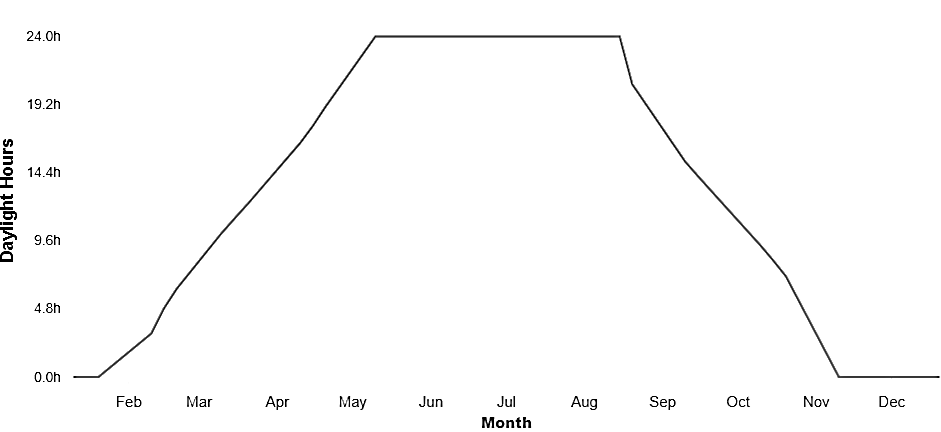
\includegraphics[width=0.8\textwidth]{figures/SOLAR_Daylight distribution.png}
    \caption{Annual daylight distribution at the EastGRIP, plotted using the DYDQI daylight simulation tool \cite{dydqi}.}
    \label{fig:Daylight}
\end{figure}

It can be seen from Figure \ref{fig:Daylight}, that the camp experiences near continuous sunlight during the active months. This displays that the camp location experiences 
a phenomenon called 'polar day' which is common within high altitude arctic regions. As a result this implies that a high yield solar energy can potentially be continuously produced 
during these months; however, as shown, the photovoltaic generation isn't viable throughout the winter 'polar night' and becomes impractical. As a result, photovoltaic generation is best suited for summer operation to maximise solar capture as solar irradiance is continuously present at the site. Panels with a low elevation and tilt become less effective as the snow deposition becomes increasingly obstructive, to address this snow shedding must be factored into the final design.

\subsubsection{Environmental Challenges}
The operation of photovoltaic systems within the arctic produce many challenges from the environment and must be critically mitigated. Strong gusts of wind M5, extremely low ambient temperature M6 and snow accumulation. As an electrical system, solar panels perform more efficiently at low temperatures; however, as a physical structure, many mechanical challenges arise from the various forces applied by wind loads and snow accumulation. The EastGRIP camp is located in an ice desert with virtually no natural wind shielding, as a consequence strong gusts can suddenly occur M5, which will be a major factor in the structural design.

\subsubsection{Concept Development and Final Panel Features}
\begin{figure}[H]
    \centering
    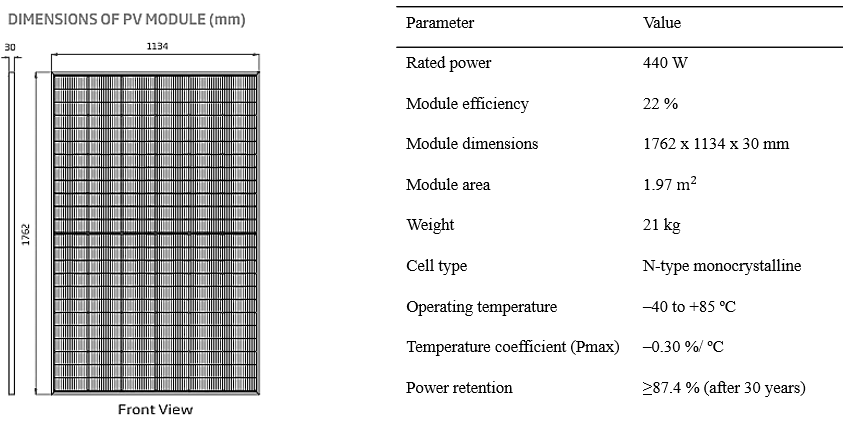
\includegraphics[width=0.75\textwidth]{figures/SOLAR_panel.png}
    \caption{Dimensions and key specifications of the Trina Vertex S+ photovoltaic module (adapted from manufacturer datasheet \cite{trina}).}
    \label{fig:Panel}
\end{figure}

Figure \ref{fig:Panel} summarises the physical dimensions and specifications for the selected Trina Vertex S+ 440W module \cite{trina}. The module utilises N-type monocrystalline technology which provides a high module efficiency (22\%) that is an advantage over conventional P-type panels. The panels have a wide operating temperature range which is suitable for Arctic deployment and a low temperature coefficient which improves the panel efficiency at low temperatures. The panel is dual glass which provides greater mechanical strength and durability, and also is bi-facially constructed. Bi-faciality provides a marginal additional rear reflected solar capture 'albedo gain' which increases the solar yield compared to conventional mono-facial modules.

\subsubsection{Panel Orientation}
Solar energy generation from photovoltaic panels depends on the tilt and azimuth (direction) of the panel specific to the location of operation. A conventional heuristic is to set the tilt according to the latitude with a seasonal adjustment:
\[
\theta \approx \phi + \phi_{season}
\]
The EastGRIP is located at [75.63° N, 35.99° W]\cite{eastgrip}, where a south facing azimuth maximises solar capture. After applying a seasonal adjustment of -15°, the tilt is approximately 60°. However, specific to the camps location such steeply tilted panels would produce many structural risks in extreme winds and storms M5: such that an additional adjustment -10° can be implemented to negate 11.5\% of the projected area and thus mechanical loading. 

Which results in a 'Adjusted orientation' : [Tilt = 50.0°, Azimuth : True south]. The complete derivation is located in Appendix \ref{app:Adjusted panel tilt derivation}. 
The impact on solar capture from the additional adjustment is assumed to be minimal, however, the 'Adjusted orientation' will be compared to a computer simulated optimised orientation to assess its validity. 

\subsubsection{Solar Energy Generation}
After theoretically deducing a panel orientation suitable for the camps specified location and environmental challenges, the PVGIS simulation tool \cite{pvgis} can be used to evaluate the adjusted orientation and calculate an optimised per annum orientation. As a result an optimised orientation per annum can be produced with its corresponding solar irradiance distribution to compare with the adjusted orientation.
\begin{figure}[H]
    \centering
    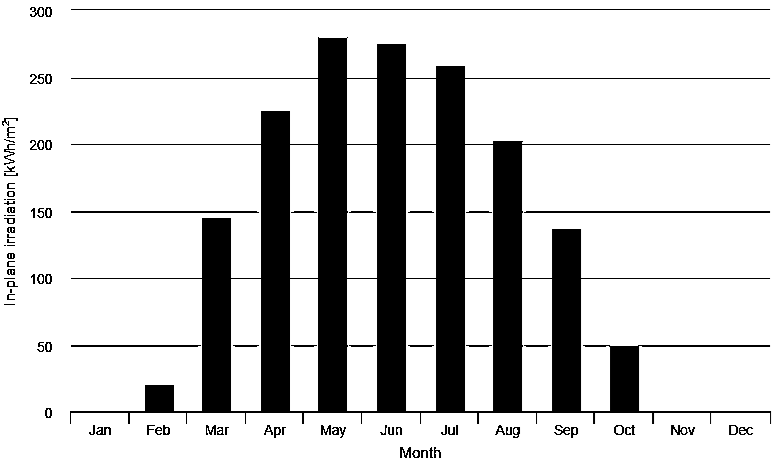
\includegraphics[width=0.8\textwidth]{figures/SOLAR_Irradiation distribution.png}
    \caption{Monthly in-plane solar irradiation distribution for the optimised orientation simulated using PVGIS \cite{pvgis}.}
    \label{fig:Irradiation}
\end{figure}
Figure \ref{fig:Irradiation} illustrates the monthly in-plane solar irradiance distribution simulated for panel orientation at the camp. The simulated distributions for both the optimised and adjusted orientations show negligible variation especially outside of the deployment period, hence a single graph can be used to represent them.

From the individual solar irradiance distribution, the predicted solar yield can be obtained by calculating the total in-plane irradiation for the operational months, followed by applying the panel efficiency coefficient for each module \cite{trina} and a typical photovoltaic system performance ratio to achieve a predicted solar energy generated during deployment as shown.
\[
\begin{aligned}
E_{solar} &= H_{ip} \times A_{total} \times \eta_{panel} \times PR \\
\\
H_{ip} &= \text{in-plane irradiation (kWh/m}^2\text{)} \\
A_{total} &= 6 \times (1.762 \times 1.134)\ \text{m}^2 \\
\eta_{panel} &= 0.22 \\
PR &\approx 0.8
\end{aligned}
\]

\begin{table}[H]
\centering
\begin{tabular}{lcc}
\toprule
Parameter & Optimised annual orientation & Adjusted orientation \\
\midrule
Tilt ($^\circ$) & 55 & 50 \\
Azimuth ($^\circ$) & $3^\circ$ (S-SW) & $0^\circ$ (True south) \\
In-plane irradiation (kWh/m$^2$) & 1243 & 1250 \\
Predicted solar energy (kWh) & 2598 & 2613 \\
\bottomrule
\end{tabular}
\caption{Comparison of the optimised and adjusted panel orientation annual parameters obtained from PVGIS simulation \cite{pvgis} followed by predicted solar yield.}
\label{tab:solar_orientation}
\end{table}

As shown in Table \ref{tab:solar_orientation}, the difference in predicted energy yield between the optimised and adjusted orientations is minimal. However, the adjusted configuration is superior as it reduces structural loading by 11.5\%, which is more suitable for the mounting design in such extreme conditions.

The minimal difference in predicted solar yield is because the simulation software optimises solar production over a full annual period, compared to actual deployment being only during Summer. The predicted annual energy yield of 2613 kWh from the 'Adjusted' configuration therefore exceeds the 'Optimised' production and therefore is utilised for the final design.

Snow accumulation is typically the dominant factor reducing photovoltaic performance in arctic environments. notwithstanding, the relatively steep 50° panel tilt combined with strong prevailing winds M5 is expected to promote continuous natural snow shedding. Consequently, snow losses are assumed to be negligible, and a typical performance ratio is applied.

\subsubsection{Mounting System}
To prepare for the arctic wind loads that will be experienced by the deployed panel configuration, the expected forces are to be calculated to determine a requirement threshold for suitable anchors to ensure stability. Each PV module is highly inclined which consequently experience significant aerodynamic drag and lift forces from strong winds M5 which concentrate at each anchor risking failure (anchor pull-out). To diminish the stress concentration by force redistribution the six solar panels will be spread across three series mounts. The calculation in Appendix \ref{app:Solar mount} determines the forces experienced and the minimum anchor dimensions to overcome with a suitable factor of safety to account for weather variability. The threshold is intended for the worst credible case of 40~kt perpendicular wind M5. Consequently, required minimum anchor capacity for any anchor selected for deployment must satisfy a cylindrical contact area DL $\geq 0.00054\,\text{m}^2$.


%----------------------------------------------------
\subsection{Wind Turbine - OM}

\subsubsection{Design Requirements and Selection Criteria}
When selecting a wind turbine for the final design, the design team had several constraints to satisfy, the most important being the environment: the turbine must operate reliably down to -30°C, tolerate gusts up to 40kt ($\approx 20.5\,\text{m/s}$) , and remain functional in snow and icing conditions. In addition, because the system is intended to be portable and field-deployable, the turbine must be compact for transport, quick to assemble on site, and cost effective. These requirements were formalised in the user requirements specification (URS) and are summarised in Table \ref{tab:urs_turbine}.

\begin{table}[h]
\centering
\caption{Turbine-relevant User Requirements Specification (URS) summary}
\label{tab:urs_turbine}
\small
\renewcommand{\arraystretch}{1.2}

\begin{tabularx}{\linewidth}{>{\raggedright\arraybackslash}p{1.2cm} >{\raggedright\arraybackslash}p{3.2cm} X}
\hline
\textbf{Code} & \textbf{Requirement} & \textbf{Turbine-relevant specification} \\
\hline
M4 & Power production & Contribute to offsetting $\approx 1\%$ of daily diesel demand ($\approx 1.7\,\mathrm{kWh/day}$) \\
M5 & Wind resistance & Safe operation up to $40\,\mathrm{kt}$ wind speed (survivability in gusts) \\
M6 & Temperature constraint & No damage / operable at $-30^\circ\mathrm{C}$ \\
M9 & Ice resistance & Turbine must tolerate or mitigate ice accretion (anti-icing / de-icing strategy) \\
M10 & Cost & Cost-effective solution consistent with project cost constraint \\
\hline
\end{tabularx}
\end{table}

\subsubsection{Turbine Selection and Final Specification}
In the feasibility stage, the initial turbine selection was the RYSE (formally known as PRIMUS) AIR 40 Off-Grid Wind Turbine, this aligned strongly with the URS for a remote, off-grid location. The AIR 40 is designed for standalone systems and includes features such as integrated charge control that supports straightforward connection into a hybrid renewable system with a shared battery bus. This is advantageous in Arctic locations, where reliability is improved by minimising components, wiring and failure points.

However, for the final design the turbine was refined to the RYSE AIR 30. While the AIR 30 is very similar to the AIR 40 in external design and setup, it is better suited to the specific EastGRIP wind conditions. This decision was not based on rated power alone, but on expected energy capture at the wind speeds that occur most frequently at the site. This can be seen in the manufacturers power curve illustrated in Figure \ref{fig:Manufacturers Power Curve}.  Manufacturer information \cite{usermanual} for the AIR 30 indicates that below approximately -10°C, the bearing grease can stiffen and the turbine may require higher wind speeds to initiate the rotation until the internal frictional heating restores normal running behaviour. For this reason, the turbine should be treated as a cold-weather-adapted component, and use low-temperature synthetic lubrication to improve start-up reliability and reduce the likelihood of seizure.

\subsubsection{Site Wind Resource Assessment}
To justify this, site wind direction and wind speed statistics were analysed. A wind rose derived from the site dataset indicates a dominant south-westerly flow (direction sector 210°-270°), shown in Figure \ref{fig:wind_rose} (wind rose for EastGRIP). This directional result suggests that a passive yaw system is sufficient when wind direction is relatively consistent.

\begin{figure}[H]
    \centering
    \hspace*{-14mm}
    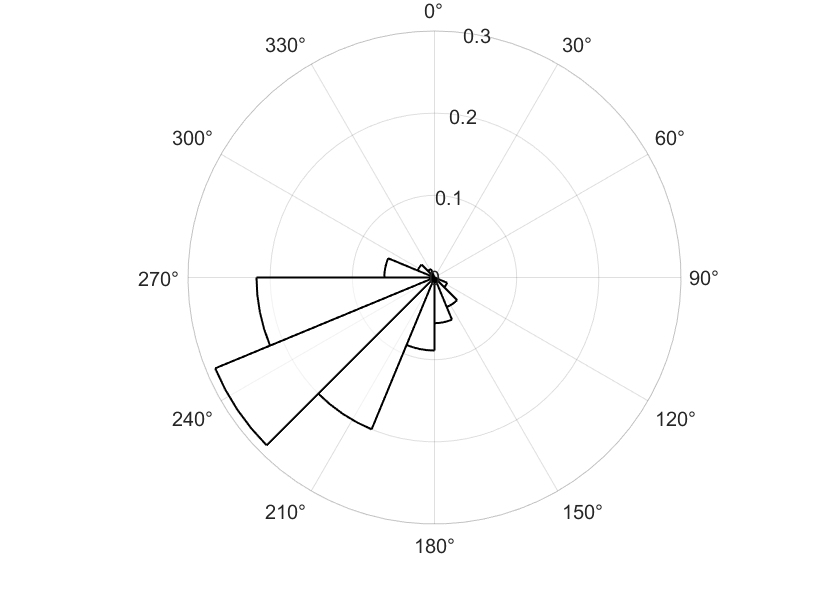
\includegraphics[width=0.9\textwidth]{windrose.png}
    \caption{Wind Rose (Direction Only) for EastGRIP}
    \label{fig:wind_rose}
\end{figure}

Wind speed behaviour was then represented using a binned histogram and a fitted distribution (Rayleigh) using a mean wind speed of 9kt, shown in Figure \ref{fig:rayleigh_distribution} (Wind speed distribution and fitted model). This provides a probabilistic representation of wind speed rather than a single deterministic average, which is essential for estimating realistic energy yield.

\begin{figure}[H]
    \centering
    \hspace*{-14mm}
    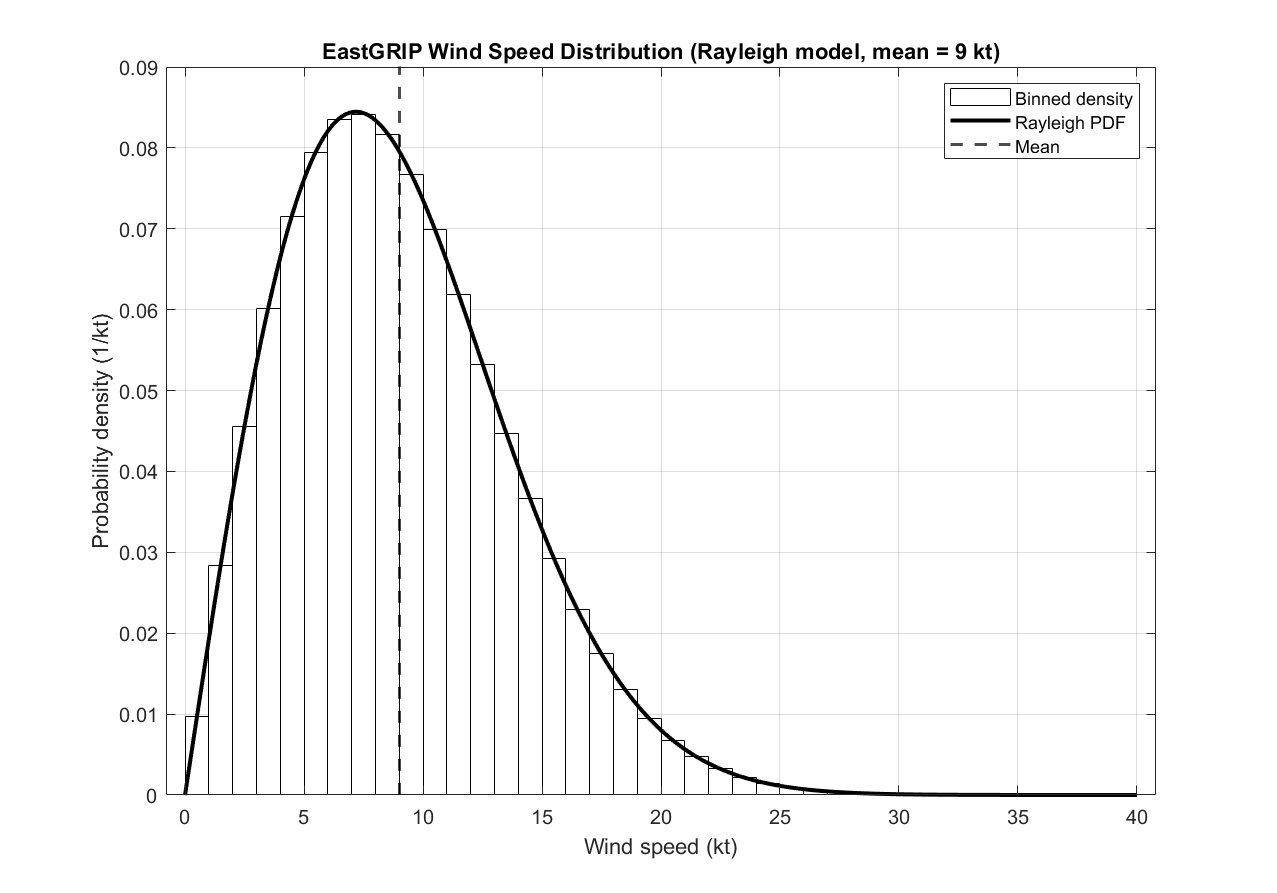
\includegraphics[width=0.9\textwidth]{figures/rayleigh distribution.png}
    \caption{Rayleigh Distribution (mean = 9 kt)}
    \label{fig:rayleigh_distribution}
\end{figure}

\subsubsection{Power Curve Modelling and Energy Yield Estimation}
To translate the wind statistics into turbine performance, the manufacturer instantaneous power curve \(P(v)\) was used to map each wind speed to electrical power output. The expected energy yield depends on how well the power curve aligns with the most frequently occurring wind speeds at EastGRIP, rather than peak power at rare high wind speeds. The AIR 30 power curve used in this analysis was digitised from the manufacturer datasheet to allow interpolation of power at intermediate wind speeds, as shown in Figure \ref{fig:Manufacturers Power Curve} (Manufacturer's power curve).

\begin{figure}[H]
    \centering

    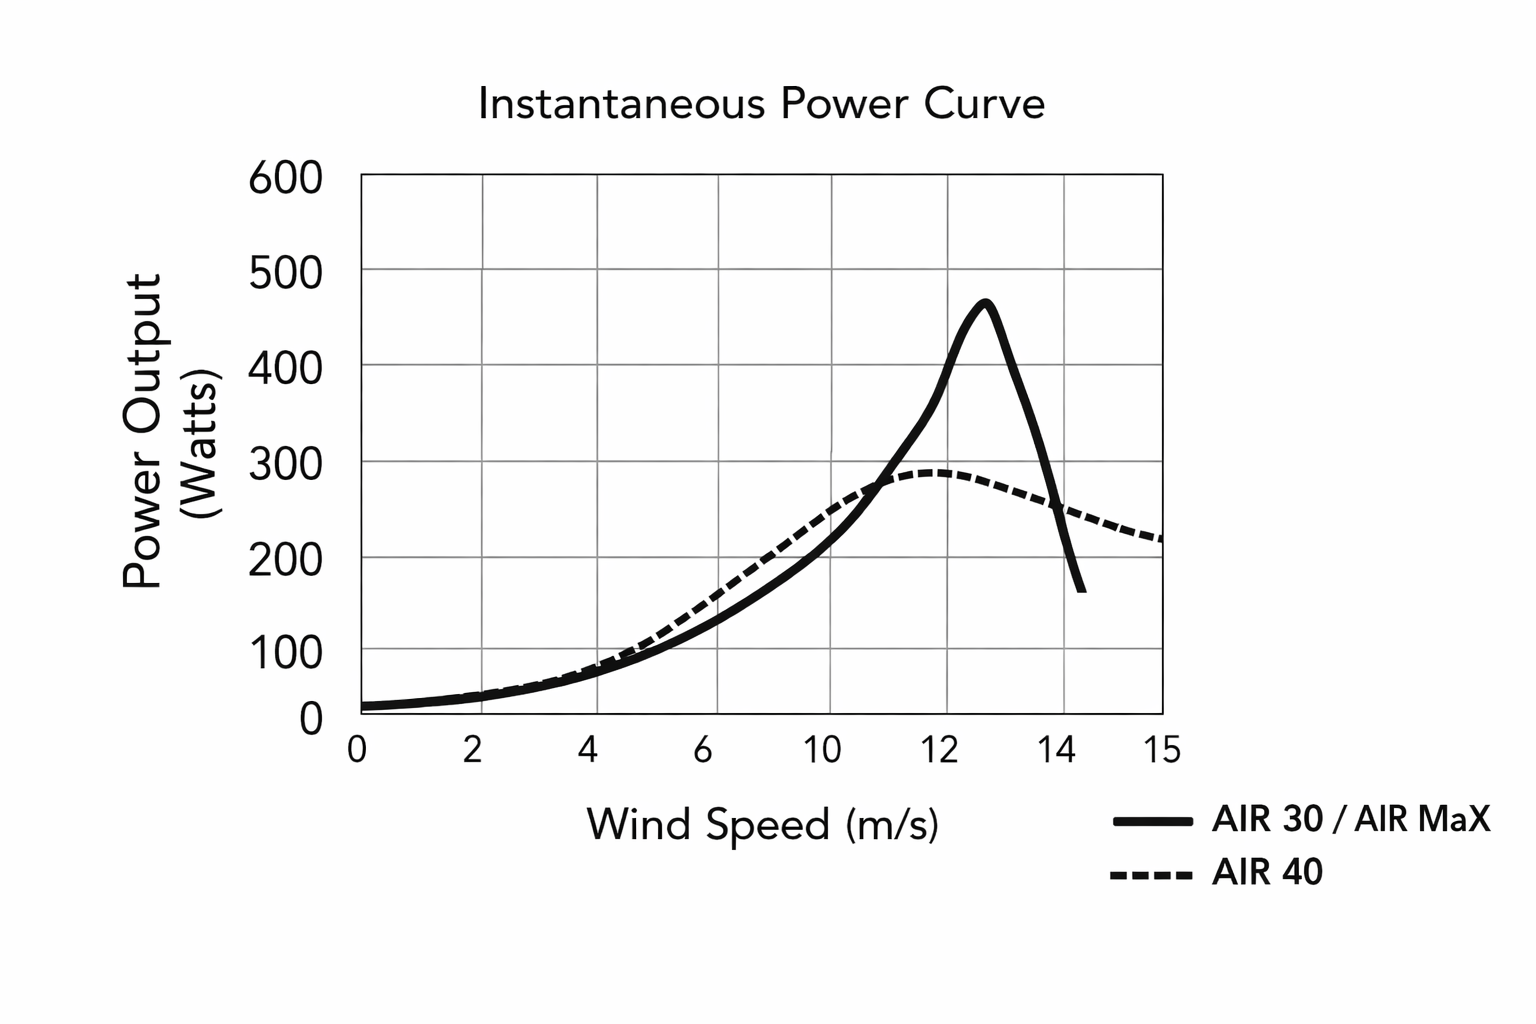
\includegraphics[width=0.8\textwidth]{figures/manufacturers power curve.png}
    \caption{Manufacturers Power Curve}
    \label{fig:Manufacturers Power Curve}
\end{figure}

A simplified expected energy estimate was then produced by weighting the turbine power output by the probability of each wind speed bin. For a given wind-speed bin \(i\) with edges \(v_{i-1}\) and \(v_i\) (and midpoint \(v_i^\ast\)), the probability of occurrence was obtained from the Rayleigh cumulative distribution function \(F_V(v)\), such that \(p_i = F_V(v_i)-F_V(v_{i-1})\). The expected energy over a period of duration \(T\) is approximated by
\[
E_T \approx T\sum_{i=1}^{N} p_i\,P(v_i^\ast),
\]
where \(P(v_i^\ast)\) is read from the digitised power curve. The contribution from each bin is therefore \(E_i = T\,p_i\,P(v_i^\ast)\), which explains the shape of Figure \ref{fig:energywindcontribution} (Contribution to expected monthly energy by wind-speed bin): although \(P(v)\) increases with wind speed, the probability of high wind speeds decreases, meaning the total energy yield is dominated by moderate wind speeds that occur most frequently. \cite{windpowerestimation}

\begin{figure}[H]
    \centering
    \hspace*{-14mm}
    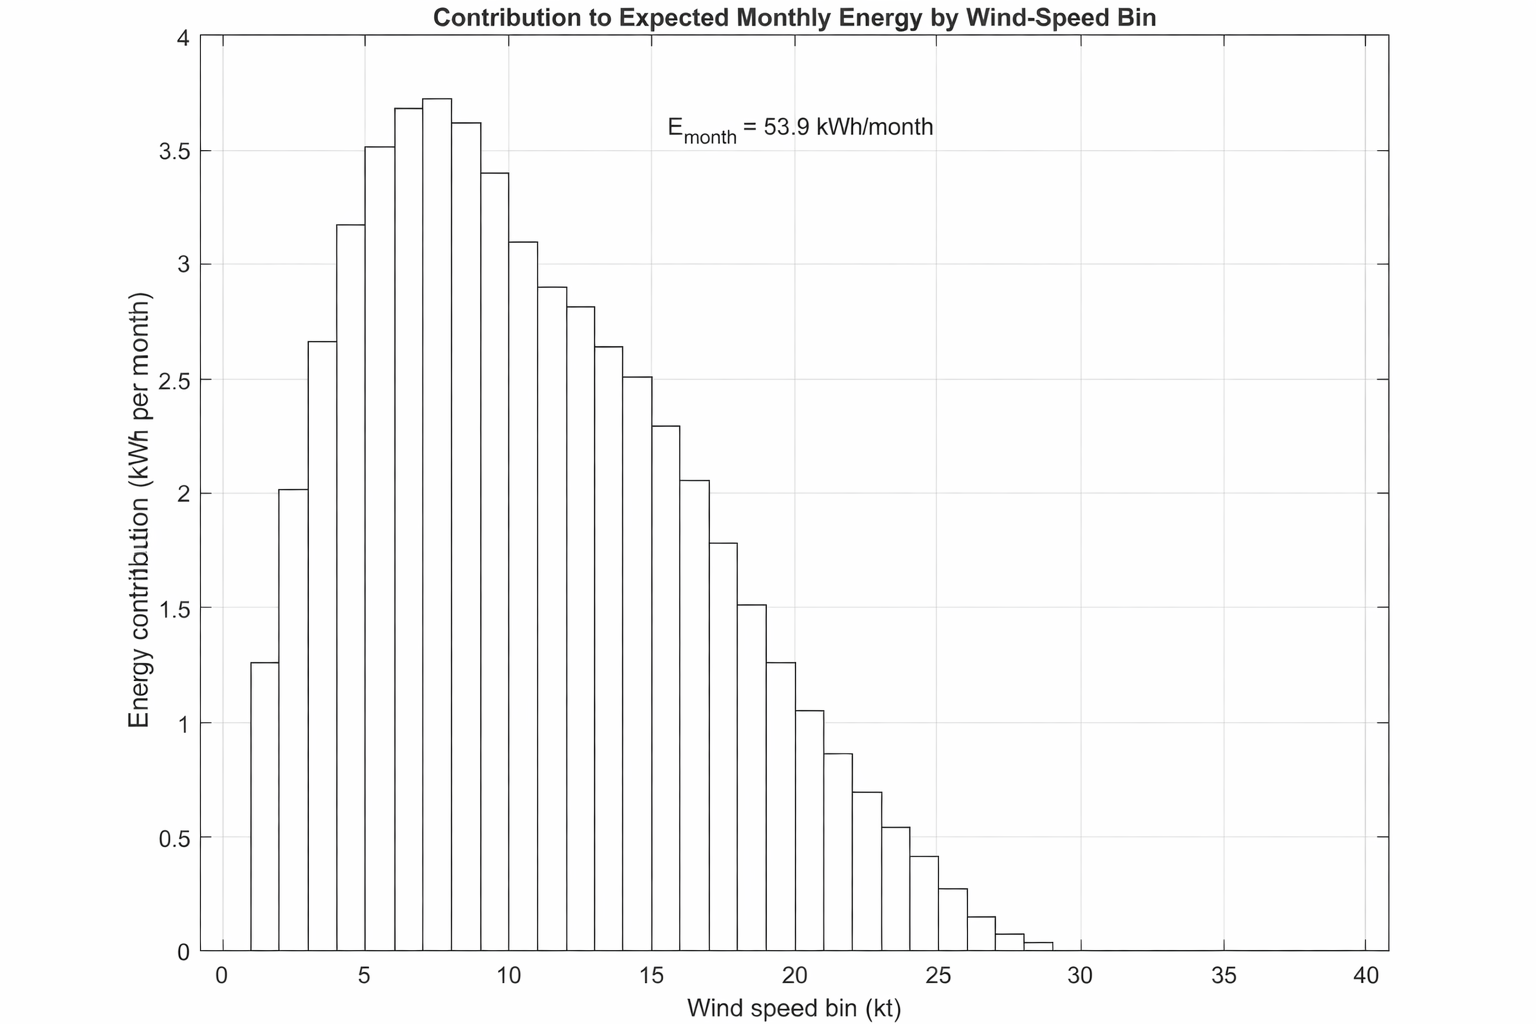
\includegraphics[width=1.1\textwidth]{figures/energy histogram plot.png}
    \caption{Wind-Speed Energy Contribution}
    \label{fig:energywindcontribution}
\end{figure}

Applying this method for EastGRIP produced an expected energy generation of \(E_{\mathrm{month}}=53.9\,\mathrm{kWh/month}\) (typical), corresponding to approximately \(E_{\mathrm{season}}=269.5\,\mathrm{kWh}\) over a \(5\)-month season, with an expected mean power of \(P_{\mathrm{exp}}\approx 75\,\mathrm{W}\). Air density effects were considered: colder Arctic temperatures increase $\rho$ , while EastGRIP’s elevation $2700~m$ reduces pressure and therefore $\rho$; these effects partially offset. As site pressure data was not available, the manufacturer power curve was used without density correction.

\subsubsection{Anti-Icing Strategy}
The project also identified icing as one of the most critical performance challenges for Arctic turbines. Ice accretion can significantly reduce aerodynamic efficiency (increased drag), leading to large reductions in power output, it can also cause imbalances to the rotor and increase vibration and structural loading. To address this, the final designs uses a passive anti-icing coating, based on a composite of polypyrrole (PPy) and PVDF applied to the turbine blades at a 1:8 ratio. This type of coating is know as superhydrophobic (reducing the water adhesion and delaying ice formation) and photothermal (absorbing solar radiation and converting it to heat).  To apply the coating, the PVDF and PPy are dissolved in a NMP solvent, then this mixture is the spray painted onto the blades and cured in a vacuum oven at 60\textbf{°}C. Evidence from literature indicates that in conditions comparable to those at EastGRIP, the photothermal polymer coating can prevent measurable ice accretion over a test duration of 60 minutes. \cite{antiicingstudy}. In the arctic circle in the summer months, nearly 24-hour solar exposure maximised the efficiency of the photothermal effects and ensuring the coating remain active, minimising icing risks. A major advantage of this coating is that it doesn't impose any additional load on the battery bank and reduces complications. However, effects due to UV radiation, particle erosion and long-term weathering can reduce the hydrophobicity over time, and performance is weakened during low-irradiance periods. For a more robust design to be used in other locations you could consider adding a small resistive leading-edge heater to the blades to assist the coating in removing ice. 

\begin{figure}[H]
    \centering
    \hspace*{-8mm}
    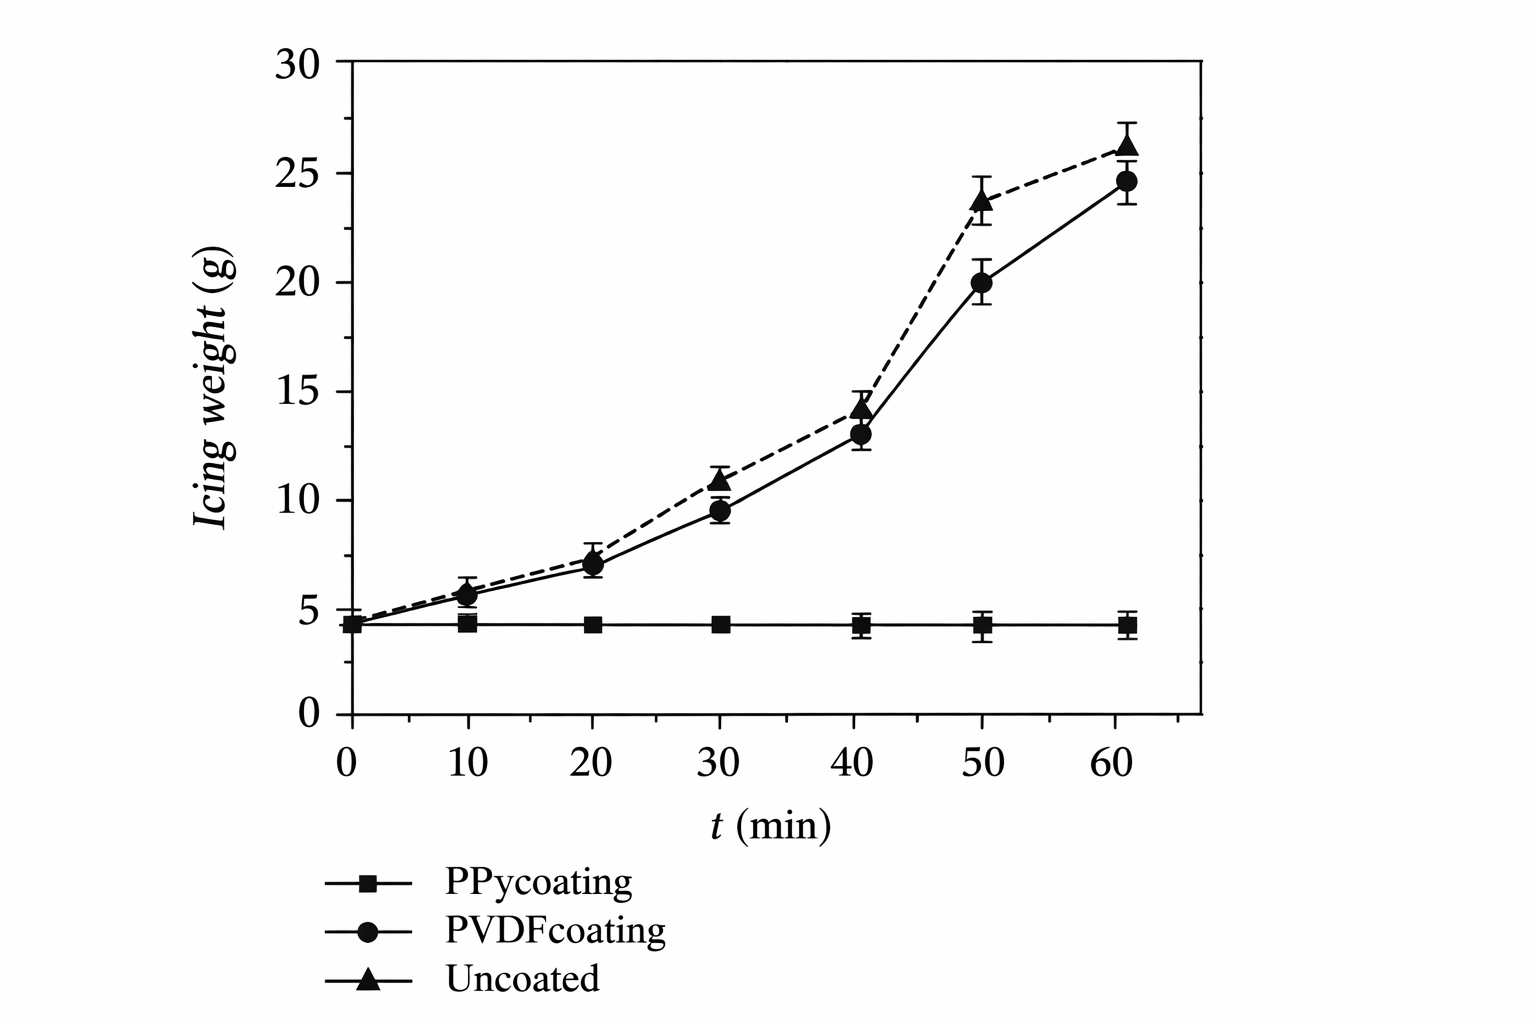
\includegraphics[width=1.1\textwidth]{figures/antiicingstudy.png}
    \caption{Anti-Icing Effectiveness}
    \label{fig:antiicingeffectiveness}
\end{figure}

\subsubsection{Turbine--Battery Interface, Charge Control and Protection}
The energy is stored by a Saft Sunica.plus nickel-cadmium (Ni-Cd) battery bank configured as a nominal 12V DC bus. Using a 12V bus is advantageous for a portable system as it is widely supported by standard off-grid system and is compatible with typical protection devices, DC loads and charging hardware. To charge the battery safely, the turbines output must be converted from AC to DC using a rectifier then controlled as to not drive the voltage above safe limits. In the system the turbine charging output is connected to the 12 V battery bus in parralell with the PV charging system, with appropriate over current protection and a DC isolation switch so the turbine can be safely disconnected for maintenance and fault isolation.  The turbine-battery-load architecture used is shown in Figure \ref{fig:system_architecture}.

Unlike solar PV, a wind turbine can overspeed if it is suddenly electrically unloaded while wind is still available. Because of this, wind turbines typically require a way of managing excess power generation when the battery is fully charged. The AIR 30 model includes an integrated charge control, intended to simplify off-grid installation; this means the turbine monitors the battery voltage and limits charging once the battery reaches a set voltage. This provides basic overcharge protection without requiring a separate wind charge controller for normal operation, reducing component count and wiring complexity, improving reliability for remote deployment. However, in more robust designs in locations with larger temperature changes, a dump-load controller can be added to absorb excess power and provide additional overspeed protection. The integrated charge controller is used as a baseline approach, with a dump-load reserved as a possible future improvement if field testing highlights the need for further high-wind speed protection.  All turbine connection to the battery bus is protected using correctly rated fuses and an accessible DC isolation. These measures reduce fire risk under fault conditions.

\subsection{Justification for Wind Turbine Inclusion}
Although the seasonal energy predictions indicates that the solar array provides the majority of the generation ($\approx$91\%), and the wind turbine contributes a smaller fraction ($\approx$9\%) under the EastGRIP summer operating scenario, inclusion of a wind turbine remain justified within the project requirements. Firstly, the role of the turbine is to improve the resilience of the power system by providing an additional source when the PV output is reduced (e.g., low irradiance, cloud and snow cover, or operation outside peak summer months), which supports the requirement to maintain a minimum level of power for important loads such as internal heaters. The turbine selected is also intentionally small-scale, reflecting the constraints of a portable pilot system so is limited by cost, size and ease of transport. Finally, the design brief emphasises that the system must both generate power and collect performance data to support future scale-up and diesel replacement. Including a wind turbine allows us to measure the wind resource at the site and understand how a turbine performs in Arctic conditions, including gust response and icing. The high solar contribution is also specific to the EastGRIP summer period with long daylight hours; at other Arctic locations and seasons with less sunlight, the wind turbine would be expected to contribute a larger proportion of the total energy.

%------------------------------------------------------
\subsection{Environmental Data Logging System (EDLS)}

\subsubsection{Objective - IK}
This project has a focus on establishing environmental data for a particular location such as the EAST grip camp, in which a variety of arctic grade environmental sensors can be implemented and combined to produce a portable autonomous data logging device (EDLS). This project aims to assess the viability of solar and wind power such that its important then to collect data on the environmental parameters which have the strongest correlation with the selected sustainable power sources. Solar irradiance, wind speed and direction sensing will be conducted. Ambient temperature is also a crucial environmental parameter as it is an important heuristic in assessing the reliability of both internal and external components in arctic regions. 

Each of the sensing components are uniquely suited best for arctic operation, compatibility between sensing subsystems can be ensured with necessary signal amplifiers and converters. Considering Musts: M6 and M8, the internal electrical components must be concealed from the environment and thermoregulated in a cabinet to maintain circuit safety and reliability to prevent damage and data blackouts. 

\subsubsection{System Infrastructure - IK}

\begin{table}[H]
\centering
\begin{tabular}{ll}
\toprule
Sensor & Parameter measured \\
\midrule
CMP3 -- Pyranometer & Solar irradiance \\
WindSonic75 -- Anemometer & Wind speed + Direction \\
DS18B20 -- Thermometer & Ambient temperature \\
\bottomrule
\end{tabular}
\caption{Environmental sensors used for data acquisition.}
\label{tab:sensors}
\end{table}

As a result the following sensors have been selected as they are durable and confine to M6, effective and manufactured for arctic applications. A block diagram can be produced to depict the required infrastructure and integration of the sensors within a single system.

\begin{figure}[H]
    \centering
    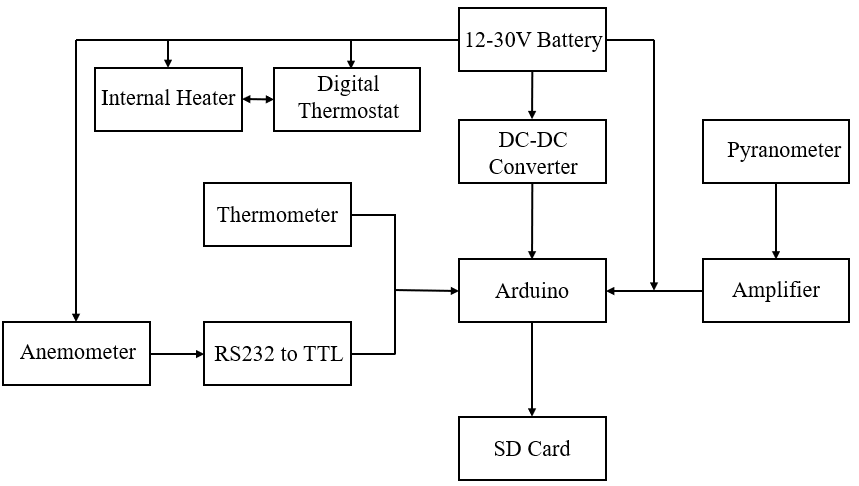
\includegraphics[width=0.85\textwidth]{figures/CIRCUIT_Block_diagram.png}
    \caption{Block diagram of the environmental sensing data logging system}
    \label{fig:Block diagram}
\end{figure}

The Block diagram displays the architecture for three distinct sensors with compatible converters to autonomously log data. the system integrates three distinct sensing devices, signal converters and amplifiers, micro controller interface, permanent data collection and storage, power distribution and voltage regulation necessary to conduct a fully autonomous data acquisition. 

A continuously operating computer to store data and provide power produces many challenges over long periods of time in the arctic and can be completely negated by implementing autonomous data processing and memory.


\subsubsection{Circuit Schematic - IK}

\begin{figure}[H]
    \centering
    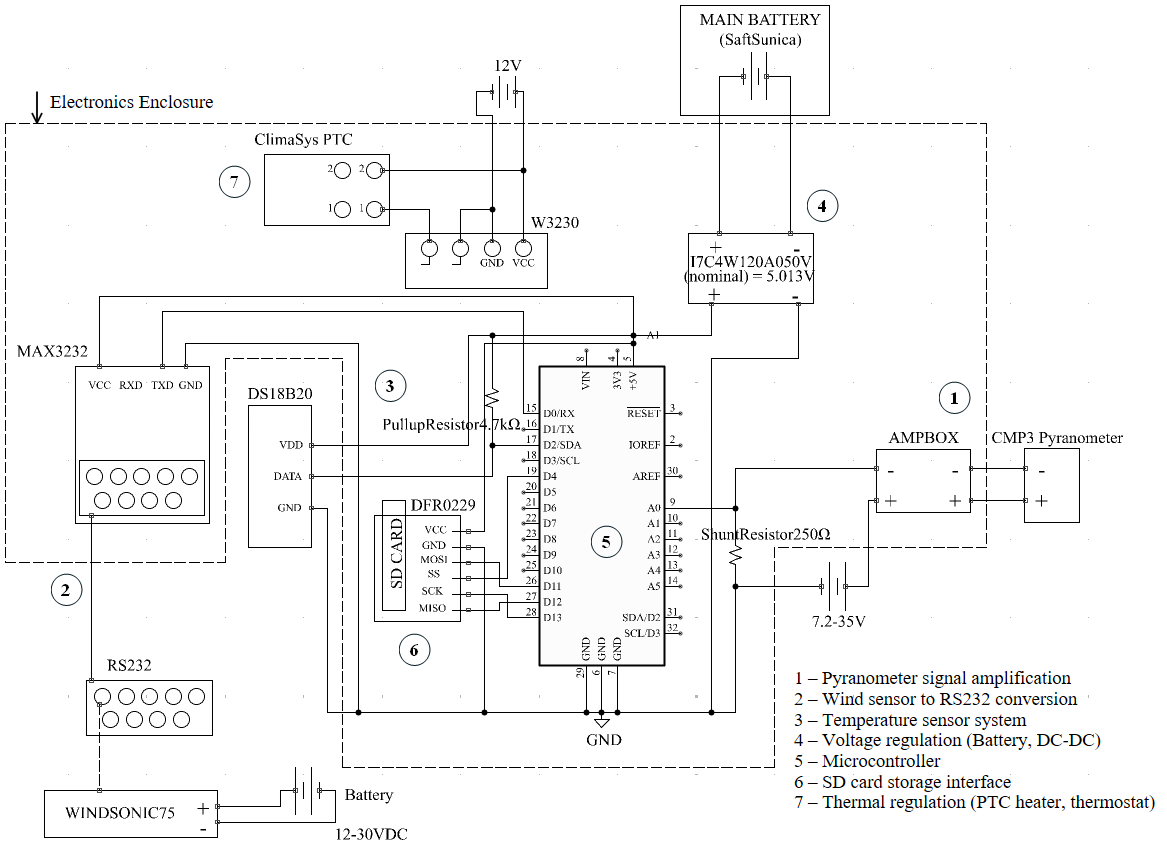
\includegraphics[width=\textwidth]{figures/CIRCUIT_Schematic.png}
    \caption{Electrical circuit schematic of the environmental sensing data logging system with subsystems (1-7) using KiCad.}
    \label{fig:CircuitSchematic}
\end{figure}

Figure \ref{fig:CircuitSchematic} portrays the circuit schematic which represents the system introduced in the block diagram. The entire electrical system is comprised of seven distinct subsystems which connect to form a complete environmental sensing data logging system. All sensors share a common ground with the microcontroller to ensure a consistent reference voltage and reliable compatibility between subsystems. To satisfy M8 requirements, each component can withstand temperatures far below 0°C as a precautionary measure despite thermoregulatory measures. Following subsections discuss the compatibility of each subsystem with corresponding schematic figures extracted from Figure \ref{fig:CircuitSchematic} with corresponding drawings from manufacturers.

\subsubsection{Solar Irradiance Sensing Subsystem - IK}
\begin{figure}[H]
    \centering
    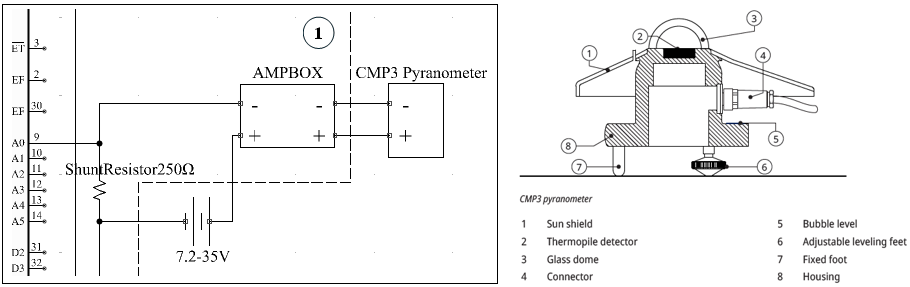
\includegraphics[width=0.8\textwidth]{figures/CIRCUIT_CMP3.png}
    \caption{Solar sensing subsystem integration (left) and CMP3 drawing from the manufacturer datasheet (right) \cite{pyranometer}.}
    \label{fig:CMP3}
\end{figure}

Solar irradiance is measured using a CMP3 pyranometer \cite{pyranometer}, which detects the total solar spectrum 300-2800 nm with a 180° field of view. The thermopile sensor converts incident solar radiation into a proportional electrical signal. A low voltage analogue signal 0-48 mV is produced which correlates to the measurement range 0-1500 W/m$^2$. The amplitude of the signal is significantly below the microcontroller input threshold hence an amplifier, AMPBOX \cite{ampbox}, is required to convert the output to  a current output (4-20mA), which applies a detectable (1-5V) across the 250Ω shunt resistor. The signal is then processed by the analogue-to-digital converter (ADC) within the microcontroller. 

\subsubsection{Wind Speed and Direction Sensing Subsystem - IK}
\begin{figure}[H]
    \centering
    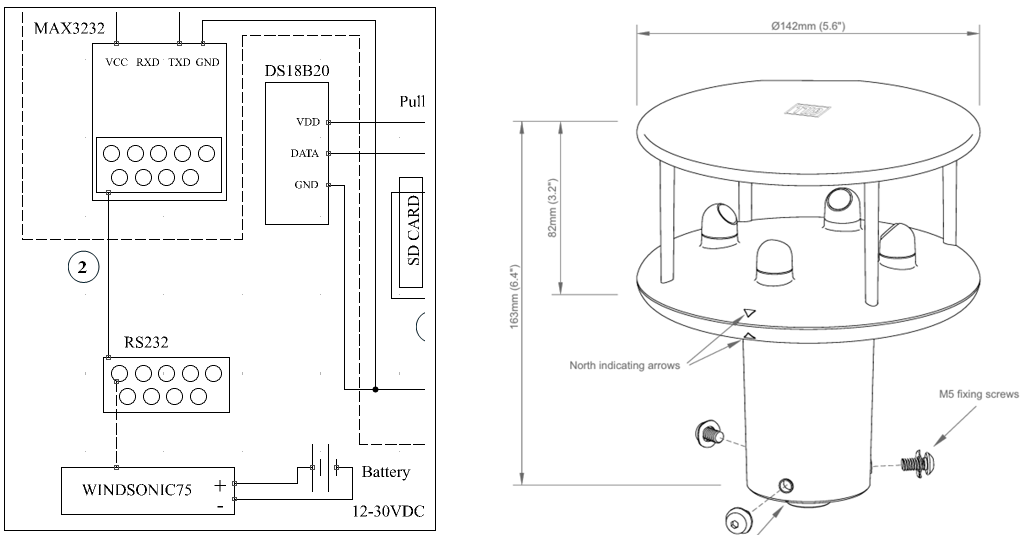
\includegraphics[width=0.8\textwidth]{figures/CIRCUIT_Wind.png}
    \caption{Wind sensing subsystem integration (left) and WindSonic75 drawing from the manufacturer datasheet (right) \cite{windsensor}.}
    \label{fig:WindSensor}
\end{figure}

Wind velocity and direction are measured using a WindSonic75 Anemometer \cite{windsensor}, which statically operates using ultrasonic technology. The sensor can measure 0-146 kt with a complete view 0-360°. The output interface RS232, requires a TTL level converter such as the MAX3232 \cite{rs232} to address the voltage disparity with the microcontroller input and ensure compatibility between interface logic. The sensor is high accuracy, corrosion free and maintenance free, which is designed for extreme climates.

\subsubsection{Temperature Sensing Subsystem - IK}

\begin{figure}[H]
    \centering
    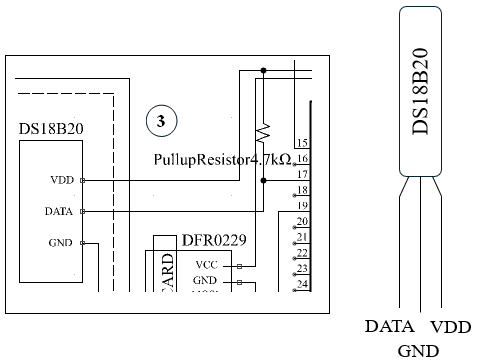
\includegraphics[width=0.4\textwidth]{figures/CIRCUIT_Temp.png}
    \caption{ Temperature sensing subsystem integration (left) and DS18B20 drawing (right)\cite{tempsensor}.}
    \label{fig:TempSensor}
\end{figure}

The DS18B20 is a stainless steel thermometer which has a measurement range of -55 to 125 °C, that is designed for arctic conditions \cite{tempsensor}. This temperature sensor is unique amongst the other sensors with a distinct 1-wire interface, exhibiting direct digital communication with the microcontroller. The digital output eliminates the need for analogue signal conditioning (converters) which eliminates the susceptibility to electrical noise interference. A suitable 4.7kΩ pullup resistor is connected to the DATA line and ensures compatibility with the microcontroller. The sensor operates with a supply voltage of 3-5V, which is provided by the Arduino. 

\subsubsection{Voltage Regulation - IK}
\begin{figure}[H]
    \centering
    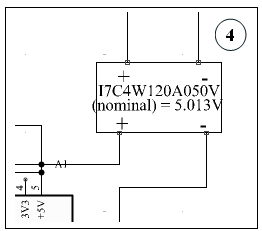
\includegraphics[width=0.25\textwidth]{figures/CIRCUIT_DCDC.png}
    \caption{Voltage regulation subsystem implementation}
    \label{fig:DCDC}
\end{figure}

The data logging system is powered by the rechargeable SaftSunica 12-30V battery supply with a nominal DC-DC converter to protect the microcontroller.  This system is primarily powered by the rechargeable battery. The battery powers the Arduino through a DC-DC converter, I7C4W120A050V \cite{dcdc}, to produce a nominal 5V supply which correctly corresponds to the Arduino +5V pin. The battery voltage is prone to fluctuations and inconsistent amplitudes of which DC-DC converter is required to ensure a stable power supply into the Arduino board. This is necessary as the microcontroller is vulnerable to fluctuating voltage which potentially could cause damage which as a result would risk the entire system.

\subsubsection{Microcontroller - IK}

\begin{figure}[H]
    \centering
    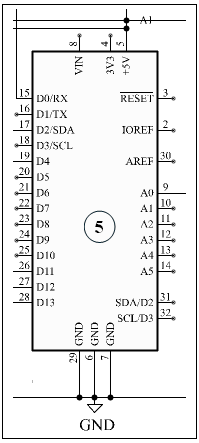
\includegraphics[width=0.2\textwidth]{figures/CIRCUIT_Mirco.png}
    \caption{Microcontroller subsystem}
    \label{fig:Mirco}
\end{figure}
The microcontroller \cite{arduino} acts as a central data processing unit between subsystems for the environmental sensing system. The Arduino UNO R3 is responsible for acquiring, processing and transmitting data for storage from the connected sensors simultaneously. The microcontroller is durable and capable of withstanding low temperatures; however, the internal heater should mitigate any risks to connected components. The Arduino processes the collected data and formats the measurements with a corresponding timestamp in a CSV line format autonomously  for extended periods of time after the program is initially embedded.

\subsubsection{Data Logging System - IK}
\begin{figure}[H]
    \centering
    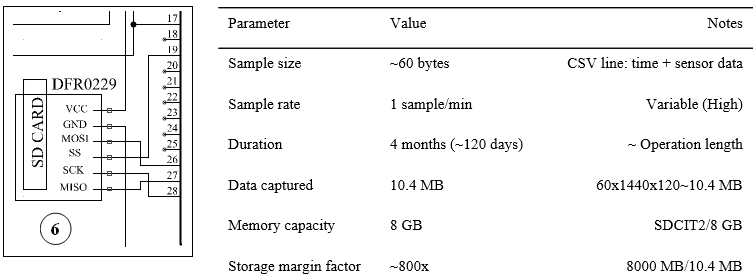
\includegraphics[width=0.8\textwidth]{figures/CIRCUIT_SD.png}
    \caption{SD card storage subsystem implementation with autonomous data logging parameters.}
    \label{fig:SD}
\end{figure}

The Autonomous data logging subsystem acts as the memory element of the system that is comprised of two components: microSD module DFR0229 \cite{sdmodule}, and a SDCIT2/8GB \cite{sdcard} industrial microSD. The module requires a 5V input with four distinct digital inputs from the microcontroller. The microSD card has a capacity margin 800x relative to the annual dataset produced. Despite this significant overprovisioning and high sample rate, these components are arctic grade and durable and their protection is crucial for the entire data logging system. Extraction of data is not frequently required as the storage margin is high (approximately 800 deployments). Therefore, to mitigate risks of data loss from unexpected damage, monthly retrieval is recommended.

\subsubsection{Thermoregulation - IK}

\begin{figure}[H]
    \centering
    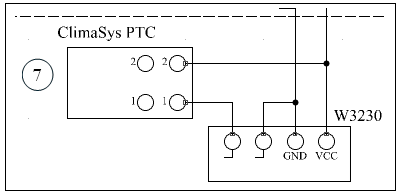
\includegraphics[width=0.4\textwidth]{figures/CIRCUIT_Heater.png}
    \caption{Thermoregulation subsystem integration}
    \label{fig:Heater}
\end{figure}

Thermoregulation ensures efficient and reliable operation of the internal electrical components and resistors and can be calibrated to adjust the desired temperature (0°C) M8. Since the heater and thermostat both fit as internal components their size was a major factor in considering low power heating.

The task is to integrate insulation to minimise the required power consumption from the heater. A ClimaSys PTC \cite{heater} can be regulated by a digital thermostat W3230 \cite{thermostat} to switch the heater off when the circuit box reaches a target ambient temperature. As the device will be deployed during summer months, it is expected that the heater will functioning for slightly more than half of the time the whole device is active.  

\subsubsection{Sensor Control Logic - CJ}

\begin{figure}[H]
\centering

\begin{minipage}{0.4\textwidth}
\centering
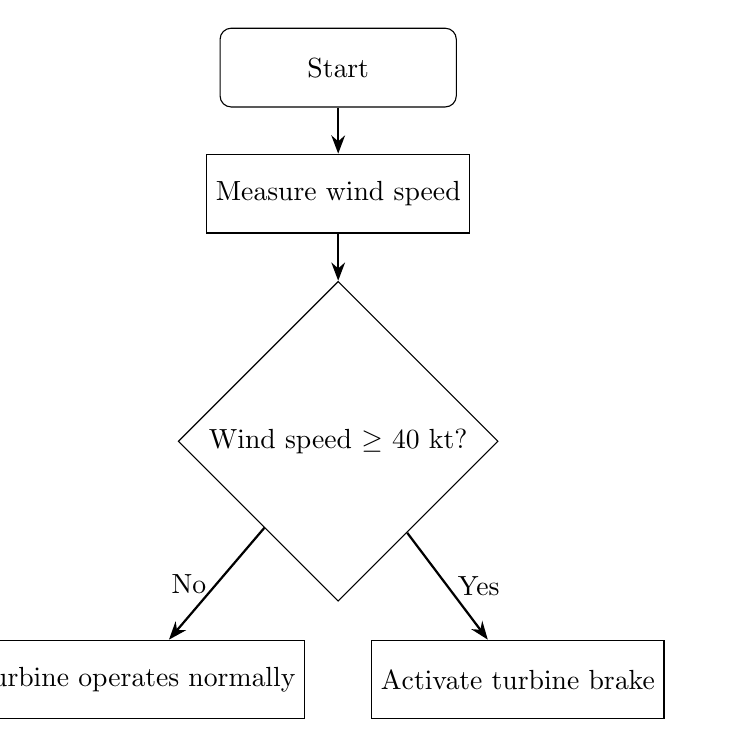
\begin{tikzpicture}[node distance=1.6cm]
\hspace*{-8mm}

\node (start) [startstop] {Start};
\node (measure) [process, below of=start] {Measure wind speed};
\node (decision) [decision, below =0.6cm of measure] {Wind speed $\geq$ 40 kt?};

\node (normal) [process, below left=1.5cm and -0.6cm of decision] {Turbine operates normally};
\node (brake) [process, below right=1.5cm and -0.6cm of decision] {Activate turbine brake};

\draw [arrow] (start) -- (measure);
\draw [arrow] (measure) -- (decision);
\draw [arrow] (decision) -- node[left] {No} (normal);
\draw [arrow] (decision) -- node[right] {Yes} (brake);

\end{tikzpicture}

\vspace{3mm}
\small (a) Turbine overspeed protection
\end{minipage}
\hfill
\begin{minipage}{0.4\textwidth}
\centering
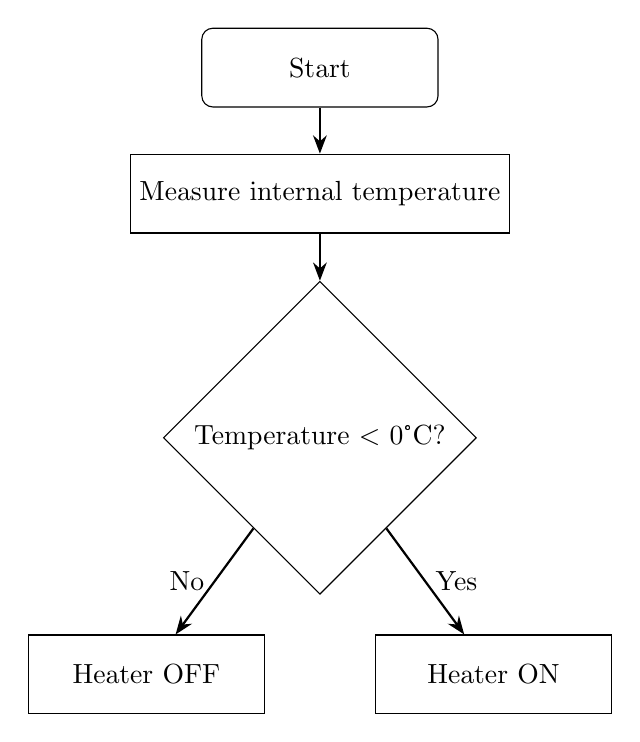
\begin{tikzpicture}[node distance=1.6cm]

\node (start) [startstop] {Start};
\node (measure) [process, below of=start] {Measure internal temperature};
\node (decision) [decision, below =0.6cm of measure] {Temperature $<$ 0°C?};

\node (off) [process, below left=1.5cm and -0.3cm of decision] {Heater OFF};
\node (on) [process, below right=1.5cm and -0.3cm of decision] {Heater ON};

\draw [arrow] (start) -- (measure);
\draw [arrow] (measure) -- (decision);
\draw [arrow] (decision) -- node[left] {No} (off);
\draw [arrow] (decision) -- node[right] {Yes} (on);

\end{tikzpicture}

\vspace{3mm}
\small (b) Internal temperature control
\end{minipage}

\caption{Simplified logical decision processes governing turbine overspeed protection and enclosure temperature regulation.}
\label{fig:sensor_logic}

\end{figure}
The turbine braking and environmental data logging subsystems incorporate internal sensor-based control logic that autonomously regulate turbine operation and electronics temperature. As both the wind turbine and digital thermostat are commercial components, the detailed control circuitry is embedded within their internal controllers. However, the logical decision processes governing their behaviour were analysed to ensure correct integration within the overall system design.

Two key logic-controlled subsystems are present: turbine overspeed protection and internal temperature regulation. The simplified decision logic implemented within the turbine and thermostat controllers is illustrated in Figure 19.

The RYSE AIR 30 turbine selected for the design includes an integrated wind-speed sensing and braking system. When wind speeds exceed the manufacturer’s safe operating threshold of 40 knots, the controller activates the turbine braking mechanism and disconnects the generator. This protects the turbine structure from overspeed damage and prevents excessive electrical loading during extreme weather conditions. Although winds above 40 kt are unlikely at the EastGRIP camp, this feature ensures the design remains viable for deployment in other locations.

Similarly, the enclosure heating system uses a digital thermostat with an integrated temperature sensor. When the internal enclosure temperature falls below 0 °C, the thermostat activates an internal heater to maintain electronics within their safe operating range. Once the temperature rises above the threshold, the heater automatically switches off.


\subsubsection{Insulation - SO}
The external temperature was taken into consideration when designing this circuit along with the components as they needed to function at these low temperatures. In order to accommodate these requirements, it was necessary to incorporate insulation and small heaters. We chose to include two small 20W heaters and polyurethane foam pads for insulation which have a very low thermal conductivity and can be cut to shape for the inside of the base. initially, it was decided to insulate and heat the entirety of the base but, after some calculations, the total heat loss from the base after including 80mm thick walls of insulation was over 150W at the minimum temperature of -40C. The calculations for this can be found in the appendix. The most viable solution was to provide insulation specifically for the smaller circuit box within the base which had a significantly smaller surface area that gave an estimated heat loss of only 22W (Found in appendix \ref{app:Insulation Calculations}).


%---------------------------------------------------
\subsection{Circuit Safety - SO}
The following circuit diagram gives a rudimentary overview of how the parts will be connected:

\begin{figure}[H]
\centering
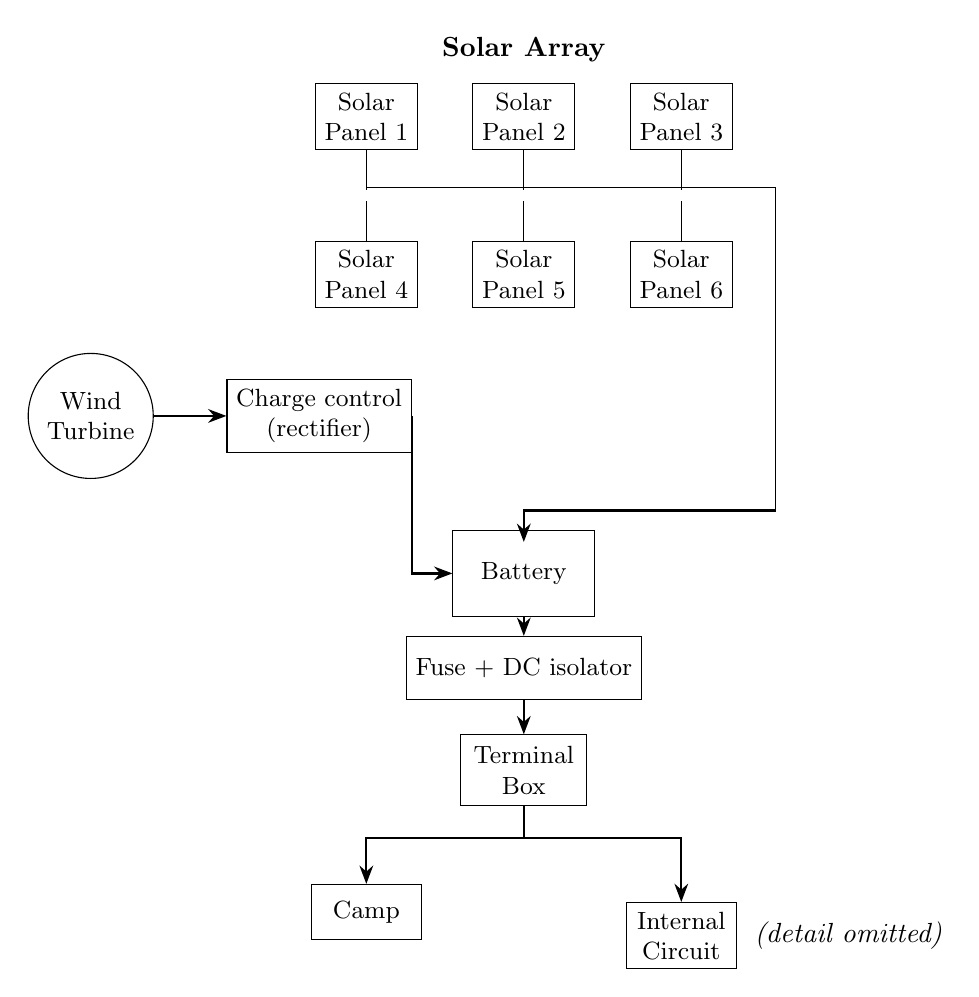
\begin{tikzpicture}[
    font=\small,
    panel/.style={draw, rectangle, minimum width=1.2cm, minimum height=0.8cm, align=center},
    battery/.style={draw, rectangle, minimum width=1.8cm, minimum height=1.1cm, align=center},
    terminal/.style={draw, rectangle, minimum width=1.6cm, minimum height=0.9cm, align=center},
    load/.style={draw, rectangle, minimum width=1.4cm, minimum height=0.7cm, align=center},
    turbine/.style={draw, circle, minimum size=1.2cm, align=center},
    arrow/.style={-{Stealth}, thick},
    line/.style={thick}
    control/.style={draw, rectangle, minimum width=2.2cm, minimum height=1.1cm, align=center},
protect/.style={draw, rectangle, minimum width=2.4cm, minimum height=0.8cm, align=center},
control/.style={draw, rectangle, minimum width=2.2cm, minimum height=0.8cm, align=center},
protect/.style={draw, rectangle, minimum width=2.4cm, minimum height=0.8cm, align=center},
]
% --- Solar Panels in 3 columns x 2 rows ---
% Top row
\node[panel] (sp1) at (0, 7)   {Solar\\Panel 1};
\node[panel] (sp2) at (2, 7)   {Solar\\Panel 2};
\node[panel] (sp3) at (4, 7)   {Solar\\Panel 3};
% Bottom row
\node[panel] (sp4) at (0, 5) {Solar\\Panel 4};
\node[panel] (sp5) at (2, 5) {Solar\\Panel 5};
\node[panel] (sp6) at (4, 5) {Solar\\Panel 6};

% Vertical wires from top row down to horizontal bus
\draw[line] (sp1.south) -- ++(0, -0.5);
\draw[line] (sp2.south) -- ++(0, -0.5);
\draw[line] (sp3.south) -- ++(0, -0.5);

% Horizontal bus between top and bottom rows at y=6.1
\draw[line] (0, 6.1) -- (5.2, 6.1);

% Vertical wires from bottom row up to horizontal bus
\draw[line] (sp4.north) -- ++(0, 0.5);
\draw[line] (sp5.north) -- ++(0, 0.5);
\draw[line] (sp6.north) -- ++(0, 0.5);

% Vertical collection wire down from bottom row panels

% Bottom horizontal bus at y=4.9

% Collect from right end of bottom bus, go down and into battery
\draw[line] (4, 6.1) -- ++(0.8, 0);
\coordinate (right_rail_top)    at (5.2, 6.1);
\coordinate (right_rail_bottom) at (5.2, 2.0);
\draw[line] (right_rail_top) -- (right_rail_bottom);
\draw[arrow] (right_rail_bottom) -| (2, 2.0) -- (2, 1.6);

% --- Wind Turbine ---
\node[turbine] (wt) at (-3.5, 3.2) {Wind\\Turbine};
% --- Charge control / rectifier block ---
\node[control] (cc) at (-0.6, 3.2) {Charge control\\(rectifier)};


% --- Battery ---
\node[battery] (bat) at (2, 1.2) {Battery};

% --- Protection block between battery and terminal box ---
\node[protect] (prot) at (2, 0.0) {Fuse + DC isolator};

\node[terminal] (tb) at (2, -1.3) {Terminal\\Box};

% Battery -> protection -> terminal box
\draw[arrow] (bat.south) -- (prot.north);
\draw[arrow] (prot.south) -- (tb.north);

% Wind turbine to battery
% Wind turbine -> charge control -> battery
\draw[arrow] (wt.east) -- (cc.west);
\draw[arrow] (cc.east) |- (bat.west);

% --- Terminal Box ---


% Battery to terminal box


% --- Outputs from Terminal Box ---
\node[load] (camp) at (0, -3.1) {Camp};
\node[load] (sc)   at (4, -3.4)  {Internal\\Circuit};

% Terminal box to Camp
\draw[arrow] (tb.south) -- ++(0, -0.4) -| (camp.north);

% Terminal box to Internal Circuit
\draw[arrow] (tb.south) -- ++(0, -0.4) -| (sc.north);

% --- Labels ---
\node[above=0.15cm of sp2, font=\bfseries] {Solar Array};
\node[right=0.1cm of sc, font=\itshape] {(detail omitted)};

\end{tikzpicture}
\caption{Simplified system architecture showing the connection between the solar array, wind turbine, battery storage, and electrical loads.}
\label{fig:system_architecture}
\end{figure}

It is vital that electrical components are handled with care, particularly in arctic conditions as snow and ice can melt near these components: potentially damaging them or injuring someone handling them. Do not connect the microcontroller and other components to a power supply until everything else has been finished. Connections into the arduino should be double checked in order to prevent a short circuit, which would damage it beyond repair, and power should only be switched on through the terminal box.
The battery can produce a significant voltage so any time it is being worked on, the worker should wear suitable protective equipment including thick gloves and eye protection. There is also a fuse included to prevent damage if a power surge from the battery did occur.

In the future, a major update is solving how the sensors are mounted and fit onto the base. Currently, they need to be attached to the top of the base and wired from around an edge of the base.

\subsection{Configuration \& Structural Support - NW}

\subsubsection{Guy Rope tensions}
To validate the stability of the structure, the worst-case loading scenario was analysed in order to determine the maximum tension in the guy ropes. The analysis was based on three key assumptions: first, the wind speed corresponds to the maximum recorded value at the EastGRIP site (40\,kn); second, wind loading is aligned with two of the guy ropes, such that only two cables resist the overturning moment; and third, the guy ropes provide the primary resistance to mast overturning about the top of the housing.

During overspeed conditions the turbine activates its internal braking system and ceases rotation. In this state the turbine behaves as a bluff body subjected to aerodynamic drag. The drag force acting on the mast--turbine assembly is approximated by:

\[
F = \frac{1}{2}\rho V^2 A C_d
\]

where $\rho$ is the air density, $V$ is the wind speed, $A$ is the projected frontal area of the turbine and mast, and $C_d$ is the drag coefficient. Using the site wind speed and air-density data, the resulting overturning moment about the top of the housing was estimated as:

\[
M = 556 \text{ Nm}.
\]

Guy ropes are typically pretensioned to prevent slack cables and to reduce dynamic loading during gusts. A pretension of approximately 300\,N was therefore applied in the design.

Under the worst-case loading condition, the maximum tension occurs in the upwind guy rope and was calculated as:

\[
T_{\text{max}} = 570 \text{ N}.
\]

The downwind rope experiences a minimum tension of approximately 30\,N, ensuring that no cables become slack during operation.

The selected guy ropes are 5\,mm diameter, $1\times19$ strand, 316-grade stainless steel cables with a rated breaking force of 19\,kN. The resulting factor of safety is therefore:

\[
FoS = \frac{19\,000}{570} \approx 33.3.
\]

This indicates a substantial structural safety margin for the guy rope system under the assumed worst-case wind loading.

\subsubsection{Ice Anchor Grounding System}
To secure the guy ropes into the ice, the guy ropes will be connected to grounding mounts. The mounts are 110\,mm long and contain two holes of diameter 22\,mm, with centre spacing of 80\,mm. These mounts are installed using two boreholes of diameter 40\,mm that will be drilled 1.5\,m into the ice, also with centre spacing of 80\,mm. 

Through the mounts and into the boreholes, two M20 coarse-thread steel anchor rods of length 1.2\,m will be inserted. Liquid water will subsequently be poured into the annular gaps between the rods and the boreholes. The rods will be held in position while the water freezes completely. This method of securing anchors within ice is known as \textit{adfreeze}.

Laboratory experiments on piles frozen into ice have reported adfreeze bond strengths between 0.2\,MPa and 0.6\,MPa for steel surfaces, depending on temperature and loading rate \cite{adfreeze}. However, because ice exhibits time-dependent creep and bond strength decreases significantly near the melting point, engineering designs typically adopt conservative allowable stresses significantly lower than peak laboratory values. Based on these considerations, a conservative shear stress of

\[
\tau = 0.1\,\text{MPa}
\]

was adopted for the stability calculations.

This method of anchoring was selected for the present design because it is inexpensive and highly reliable, and it is commonly used in installations such as the EastGRIP camp. Personnel responsible for assembling the system are therefore expected to be familiar with the procedure and to have access to the required tools, including a 40\,mm ice auger already available at the camp.

The pullout force of an adfreeze anchor can be approximated by:

\[
F = \tau (\pi D L)
\]

 The shear force acts at the interface between the refrozen water and the surrounding permanent ice; therefore the relevant diameter is the borehole diameter of 40\,mm.

Using these assumptions, the maximum allowable pullout force is

\[
F_{\text{max}} = 30\,\text{kN}.
\]

The maximum pullout force resulting from the guy rope tension calculations is 391\,N. The resulting factor of safety is therefore:

\[
FoS = \frac{30\,000}{391} \approx 76.8.
\]

This indicates that the proposed anchoring system provides a very large safety margin, making this simple installation method highly reliable for the intended application.

Adfreeze anchors are particularly effective in Arctic environments because the low ambient temperatures increase the bond strength at the steel--ice interface and limit creep deformation in the surrounding ice, allowing the frozen bond to sustain high shear resistance over extended periods.


%-------------------------------------------------------
\subsection{Bill of Materials - CJ/OM/SO/IK/NW}

\begin{table}[H]
\centering
\caption{Bill of Materials -- Primary Components}
\label{tab:bom_primary}
\begin{tabular}{lcrc}
\toprule
Component & Quantity & Unit Price (£) & Reference\\
\midrule
RYSE AIR 30 turbine & 1 & 1195 & \cite{windturbine}\\
Saft Sunica.plus batteries & 6 & 1206 & \cite{Battery Final}\\
Trina 440 W Vertex S+ panels & 6 & 381 & \cite{trina}\\
ECO-WORTHY Mounting Bracket & 3 & 677 & \cite{ECO-WORTHY Mounting Bracket}\\
PT50-6 mast & 1 & 1200 & \cite{Pole}\\
\midrule
Total: &  & $\approx$ 4728 \\
\bottomrule
\end{tabular}
\end{table}


\begin{table}[H]
\centering
\caption{Bill of Materials -- Base (Machined Parts)}
\label{tab:bom_base_machined}
\begin{tabular}{lcrc}
\toprule
Component & Quantity & Unit Price (£) & Reference\\
\midrule
90° angle brackets for 2 M18 bolts & 24 & 0.20 & \cite{Carbon Steel}\\
Guy rope groundings & 4 & 0.10 & \cite{Carbon Steel}\\
Base supports & 4 & 115.00 & \cite{Carbon Steel}\\
Housing base plate & 1 & 490.00 & \cite{Carbon Steel}\\
Housing top plate & 1 & 470.00 & \cite{Carbon Steel}\\
Long housing side plates & 2 & 300.00 & \cite{Carbon Steel}\\
Short housing side plates & 2 & 290.00 & \cite{Carbon Steel}\\
Polypyrrole (PPy) & 2g & 47.77 (fractional) & \cite{PPy}\\
PVDF Powder & 16g & 54.92 (fractional) & \cite{PVDF Powder}\\
NMP Solvent & 250ml & 42.50 (fractional) & \cite{NMP Solvent}\\
\midrule
Total: &  & $\approx$ 1810.49 \\
\bottomrule
\end{tabular}
\end{table}


\begin{table}[H]
\centering
\caption{Bill of Materials -- Base (Off-the-Shelf Components)}
\label{tab:bom_base_ots}
\begin{tabular}{lcrc}
\toprule
Component & Quantity & Unit Price (£) & Reference\\
\midrule
M18 partially threaded bolts (17\,mm unthreaded, 35\,mm threaded) & 96 & 1.10 & \cite{fasteners}\\
M18 nuts & 120 & 0.35 & \cite{fasteners}\\
M20 coarse thread bar steel rods (shaft $>$1.2\,m) & 20 & 12.00 & \cite{fasteners}\\
5\,m length, 5\,mm dia., 1x19, 316 SS cable & 4 & 25.00 & \cite{Cables}\\
M18 partially threaded bolts (42\,mm unthreaded, 38\,mm threaded) & 24 & 1.20 & \cite{fasteners}\\
M5 guy rope clamps & 4 & 1.50 & \cite{Cables}\\
M5 guy rope fastening clips & 8 & 0.80 & \cite{Cables}\\
120mm outer diameter polyurethane Sealing ring & 1 & 15.00 & \cite{Cables}\\
Electrical Box & 1 & 16.82 & \cite{enclosure}\\
\midrule \\
Total: &  & $\approx$ 73.77 \\
\bottomrule
\end{tabular}
\end{table}


\begin{table}[H]
\centering
\caption{Bill of Materials -- Circuit \& Sensors}
\label{tab:bom_circuit}
\begin{tabular}{lcrc}
\toprule
Component & Quantity & Unit Price (£) & Reference\\
\midrule
Kipp \& Zonen CMP3 Pyranometer & 1 & $\approx$ 750.00 & \cite{pyranometer}\\
Kipp \& Zonen AMPBOX Signal Amplifier & 1 & $\approx$ 500.00 & \cite{ampbox}\\
WindSonic 75 Ultrasonic Anemometer & 1 & $\approx$ 1200.00 & \cite{windsensor}\\
MAX3232 RS232 to TTL Converter & 1 & 3.00 & \cite{rs232}\\
DS18B20 Waterproof Temperature Sensor & 1 & 15.00 & \cite{tempsensor}\\
TDK i7C4W012A050V DC-DC Converter & 1 & 45.00 & \cite{dcdc}\\
Arduino Uno Rev3 & 1 & 15.00 & \cite{arduino}\\
DFRobot Micro SD Card Module & 1 & 4.60 & \cite{sdmodule}\\
Kingston Industrial SD Card & 1 & $\approx$ 25.00 & \cite{sdcard}\\
ClimaSys PTC 20W heater & 1 & $\approx$ 30.00 & \cite{heater}\\
Digital Thermostat Controller & 1 & 9.00 & \cite{thermostat}\\
250~$\Omega$ Shunt Resistor & 1 & negligible & n/a \\
4.7~k$\Omega$ Resistor & 1 & negligible & n/a\\
\midrule
Total: &  & $\approx$ 2597.00 \\
\bottomrule
\end{tabular}
\end{table}

The total predicted cost of this project is $\approx\pounds\,9{,}209 \pm 5\%$ accounting for price fluctuations.

%--------------------------------------------------
\section{Design for Manufacture - TB} 
\subsection{Production Volume}
The proposed renewable energy system is made specifically to be deployed in remote research facilities rather than for high-volume commercial production. The design has therefore been developed with small production volumes in mind, where only a minute number of units would be manufactured for specific Arctic research installations.

This low-volume production influenced several design decisions. Notably, the system has been designed to avoid complex manufacturing processes that involve expensive dedicated tooling such as casting moulds or injection moulding dies. Instead, the main structural components are built using simple machining operations and modular assemblies, which allows the system to be made economically even at small production volumes.

The design also had to prioritise modularity due to transportation restraints. This allowed individual elements to be manufactured independently and would then be assembled during the final integration stages. This method simplifies the manufacturing process and maintenance, in addition to transportation. Moreover, if any element of the build is damaged during the transport or during operations, only the affected component needs to be replaced rather than the entire structure.

Since Arctic research stations are often isolated and therefore complicated to access, the opportunities for maintenance are limited, this also explains why the system needs to be easy to assemble and disassemble. This requirement influenced the decision of using bolted structural components and standardised mounting interfaces throughout the design. 

\subsection{Manufacturing Methods}
The structural housing and support frame were designed using HSLA structural steel plate construction as it allows for straightforward manufacturing with conventional machining methods. 

The structural system consists of multiple machined elements developed through CAD modelling, including:

\begin{itemize}
\item Housing base plate
\item Housing top plate
\item Long housing side plates
\item Short housing side plates
\item Base supports
\item 90° angle brackets
\item Guy-rope grounding components
\end{itemize}

\medskip

\begin{figure}[H]
    \centering
    \begin{minipage}[t]{0.48\textwidth}
        \centering
        \includegraphics[width=\linewidth]{figures/Guy rope grounding plate.PNG}
        \caption*{\textbf{Guy rope grounding plate}}
    \end{minipage}
    \hfill
    \begin{minipage}[t]{0.48\textwidth}
        \centering
        \includegraphics[width=\linewidth]{figures/housing base plate.PNG}
        \caption*{\textbf{Housing base plate}}
    \end{minipage}
    \caption{CAD representation of the structural housing assembly showing the base plate and guy-rope grouding plate.}
\end{figure}



\textcolor{gray}{CAD models of the structural components produced by Nicholas Wright. All of these CAD renditions can be found in section \ref{app:Machined Part Schematics} in the Appendix.}

\medskip

To generate a complete rendition of the structure and to verify geometric compatibility with the supporting structure, the commercially obtained elements of the design were also made, including:

\medskip

\begin{itemize}
\item Rutland 1200 Windcharger turbine
\item Clark Masts PT50-6 telescopic mast
\end{itemize}

\textcolor{gray}{CAD models of the turbine and mast produced by Timothee Breabout.}

\medskip


All of these parts have the advantage of being easily producible through CNC milling, drilling and tapping operations. CNC machining provides sufficient precision to produce the desired mounting holes, structural interfaces and fastening points whilst still keeping repeatable manufacturing quality.

Most components are designed as simple flat plates and brackets which drastically reduces machining complexity and the amount of waste produced. Flat plate geometry also has the advantage of allowing the components to be cut directly from steel plate stock before being cut down to the final dimensions.

The use of machined plates rather than the usual welded structures makes manufacturing and transportation much simpler as the individual plates can be packed efficiently on the aircraft pallet specified in the design requirements. The final product can then easily be assembled on site using standard fasteners.

\subsection{Tooling and Assembly}
A key objective of the design for manufacture strategy was to make the need for specialised tooling as minimal as possible. Indeed, since the expected production volume is small, using custom production tooling would drastically increase manufacturing costs without providing much meaningful efficiency benefits.

The main tooling required for manufacturing the various structural components are standard CNC machining equipment. CNC milling machines are used to make the housing plates, brackets and base supports. The typical machining operations include:
\begin{itemize}
\item Plate cutting and profiling
\item Drilling of mounting holes
\item Thread tapping for fasteners
\item Machining of structural interfaces
\end{itemize}

All of these operations simply require standard milling cutters and drilling tools that are commonly found in most engineering workshops. 

The required tooling elements for assembly are also minimal. The system was designed so that all the structural components could be assembled using standard mechanical fasteners and basic hand tools that can easily be found on any exploration site, such as spanners and hex keys. This approach ensures that the device can easily be assembled but also fixed in the field if necessary.

\subsubsection{Assembly - NW}
The base housing consists of 6 plates arranged into a cube. Two opposite sides of the cube are longer and two opposite sides are shorter. The side plates sit on top of the base plate and below the top plate.
\begin{figure}[H]
    \centering
    \begin{minipage}[t]{0.48\textwidth}
        \centering
        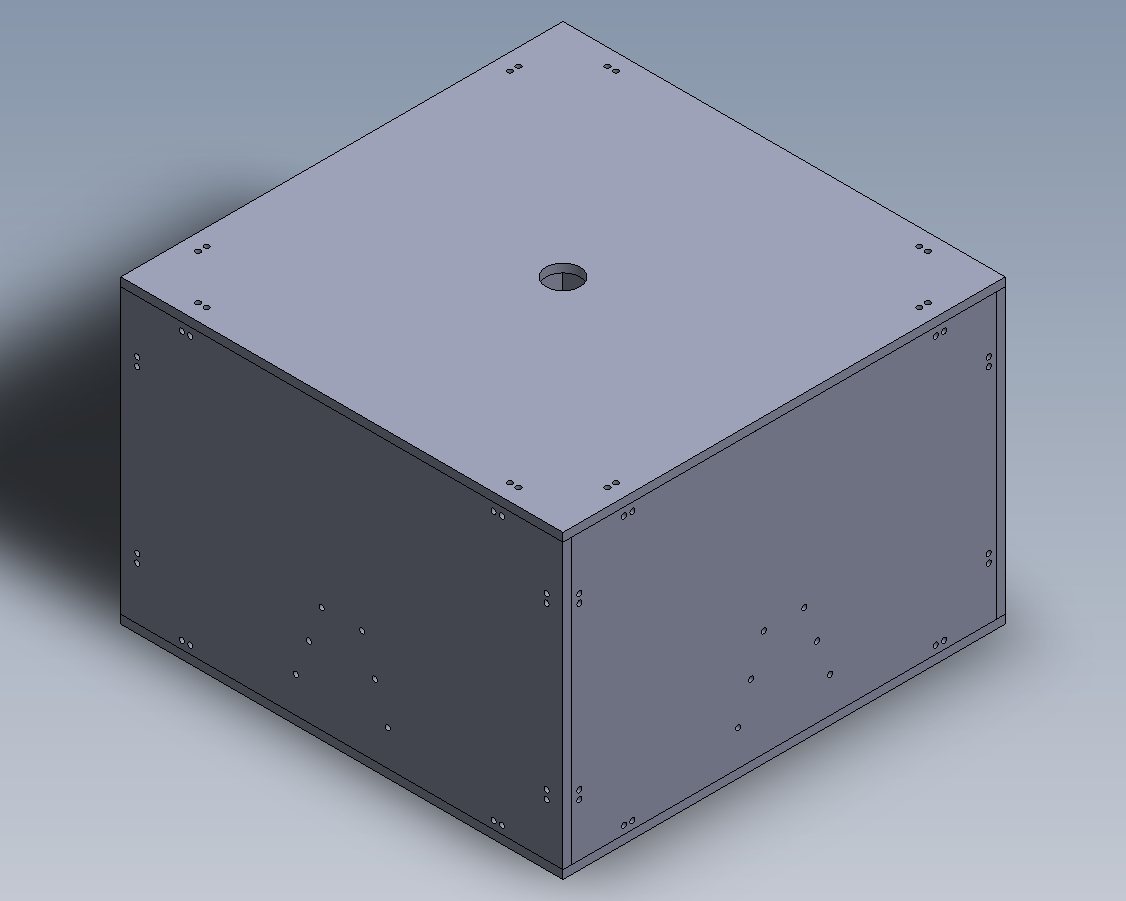
\includegraphics[width=\linewidth]{figures/housing_cube_not_exploded[1].png}
        \caption{House Cube Not Exploded}
    \end{minipage}
    \hfill
    \begin{minipage}[t]{0.48\textwidth}
        \centering
        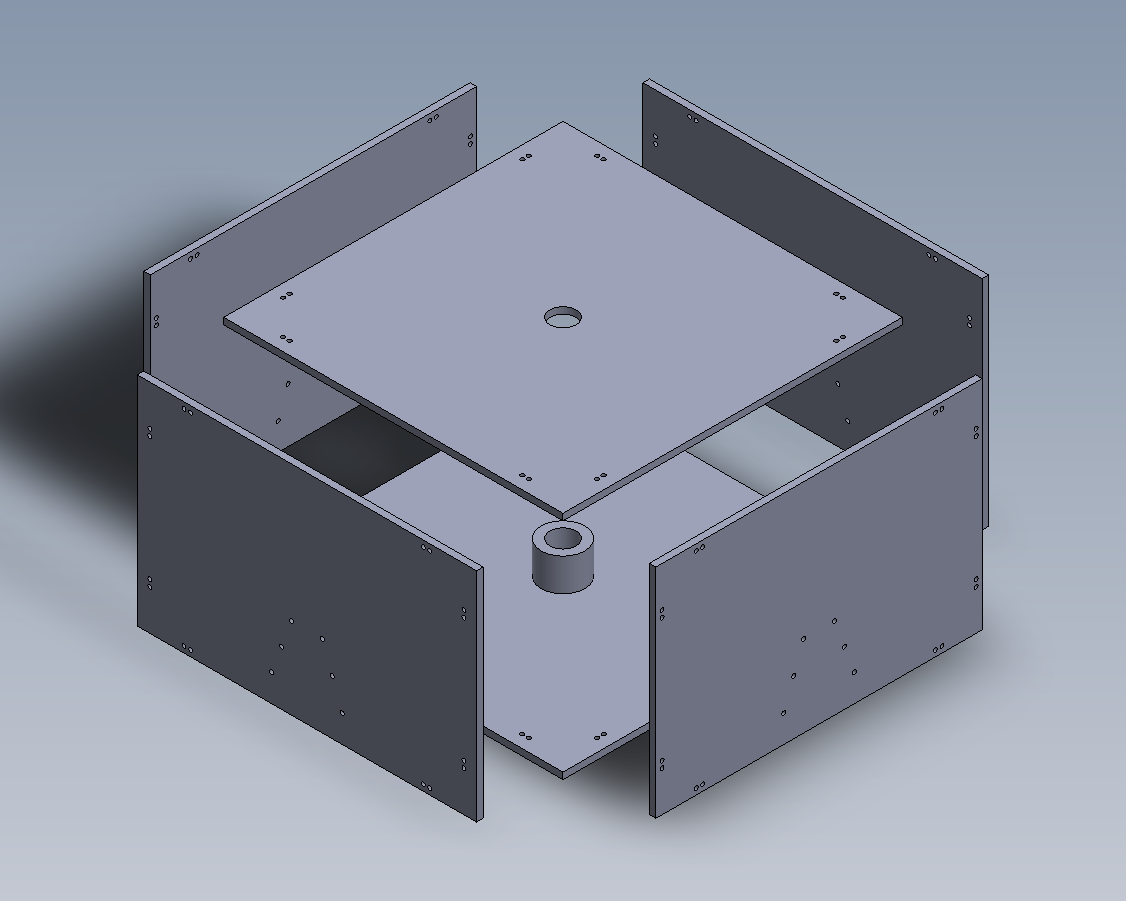
\includegraphics[width=\linewidth]{figures/housing_cube_exploded[1].png}
        \caption{House Cube Exploded}
    \end{minipage}
\end{figure}

 Each plate is attached at 90 degrees to its adjacent plates by two 90-degree angle brackets. The brackets are fastened by 4 M18 partially threaded bolts, and in turn 4 M18 nuts.
\begin{figure}[H]
    \centering
    \begin{minipage}[t]{0.48\textwidth}
        \centering
        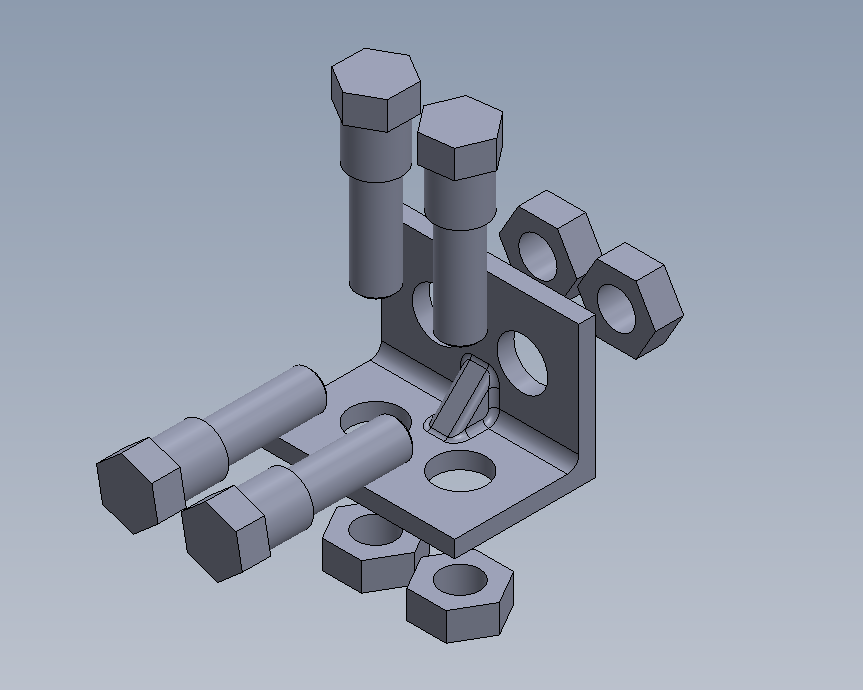
\includegraphics[width=\linewidth]{figures/bracket_asembly[1].png}
        \caption{Bracket Assembly}
    \end{minipage}
    \hfill
    \begin{minipage}[t]{0.48\textwidth}
        \centering
        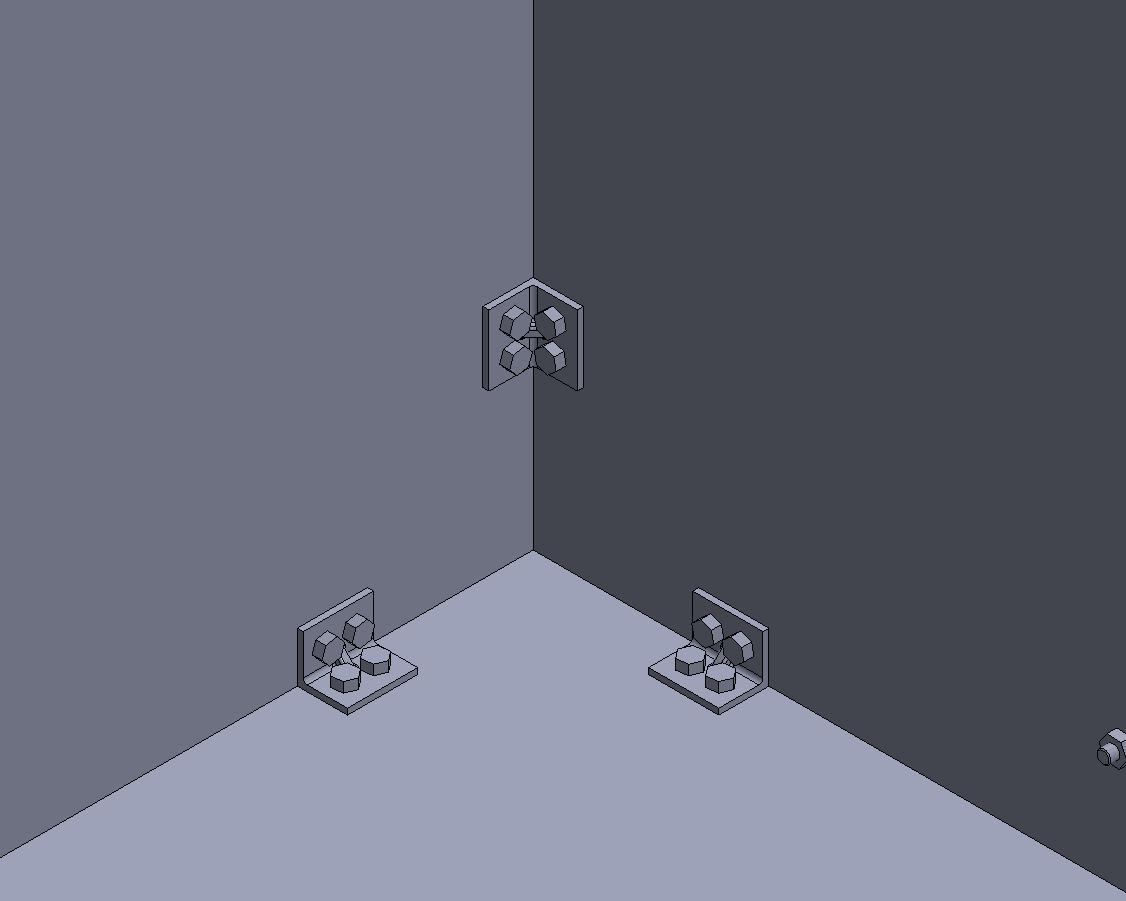
\includegraphics[width=\linewidth]{figures/housing_side_fastenings[1].png}
        \caption{House Side Fastenings}
    \end{minipage}
\end{figure}

Each side of the housing cube is supported by a base support. The base supports are attached to the side plates by 6 M18 partially threaded bolts and in turn 6 M18 nuts. The base supports will be anchored into the ice in the same manner as the Guy rope groundings (discussed earlier in section 3.5.2), using M20 rods as adfreeze anchors.
\begin{figure}[H]
    \centering
    \begin{minipage}[t]{0.48\textwidth}
        \centering
        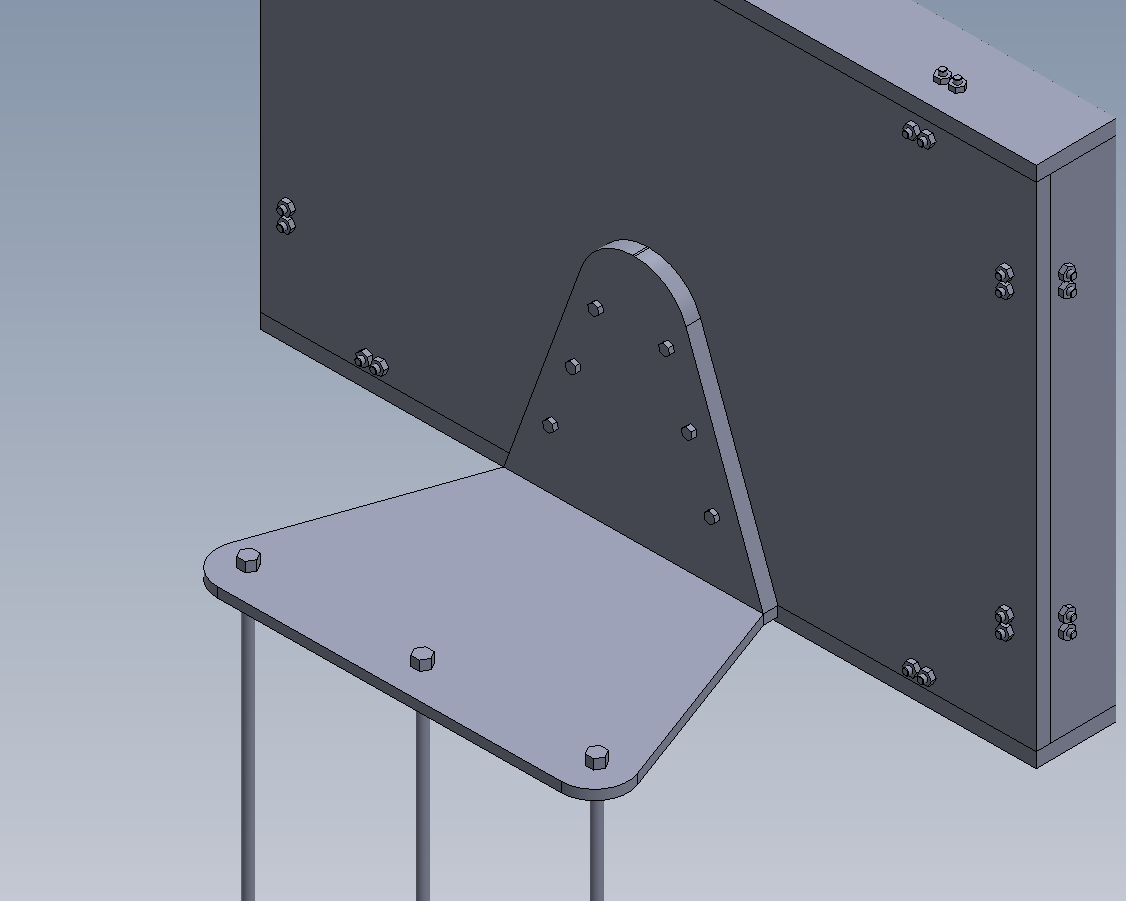
\includegraphics[width=\linewidth]{figures/base_suport_connections[1].png}
        \caption{Base Support Connections}
    \end{minipage}
\end{figure}

The base plate within the housing has a hollow cylindrical protrusion that the mast will sit within. The top plate has a circular hole that the mast can be inserted through, and the hole will in turn be sealed by a polyurethane sealing ring.  
\begin{figure}[H]
    \centering
    \begin{minipage}[t]{0.48\textwidth}
        \centering
        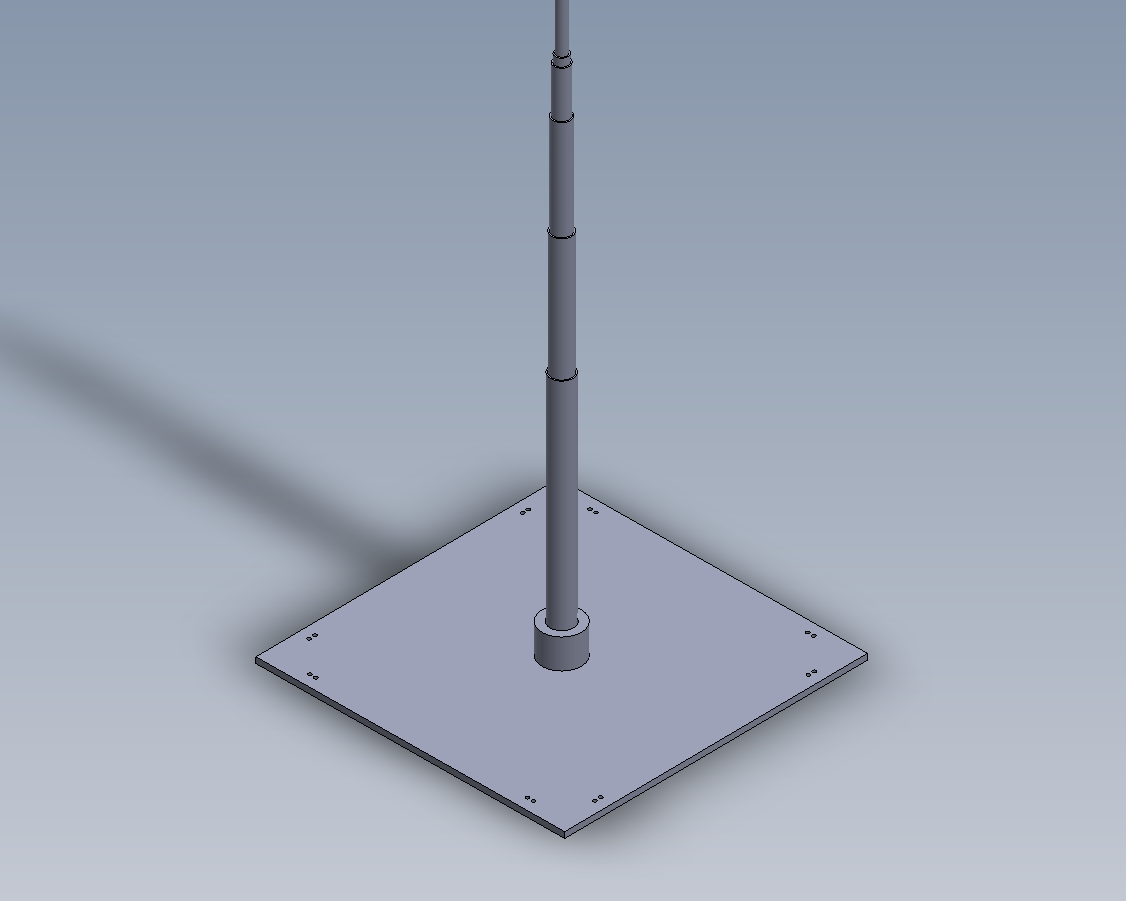
\includegraphics[width=\linewidth]{figures/base_plate_with_mast[1].png}
        \caption{Base Plate With Mast}
    \end{minipage}
    \hfill
    \begin{minipage}[t]{0.48\textwidth}
        \centering
        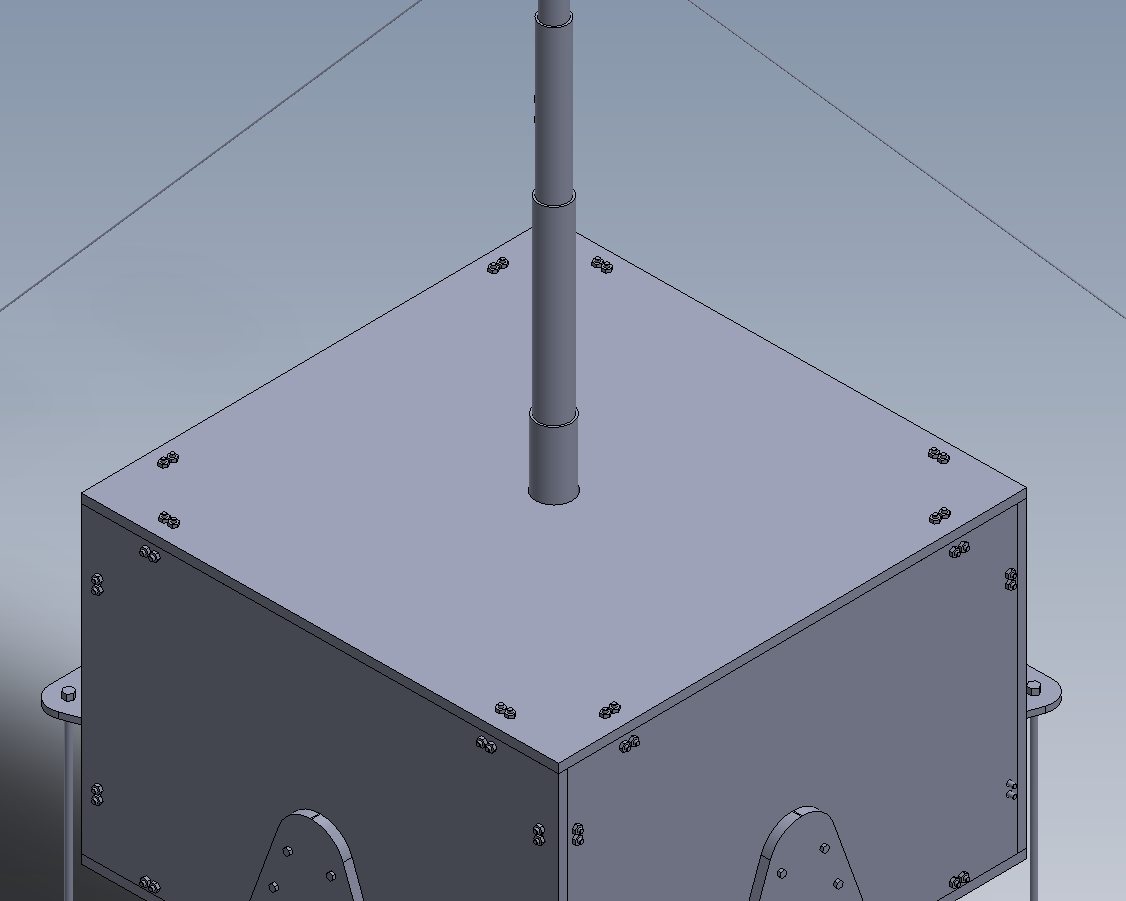
\includegraphics[width=\linewidth]{figures/top_plate_hole[1].png}
        \caption{Top Plate Hole}
    \end{minipage}
\end{figure}

The turbine attaches to the top of the mast using the standard 48mm diameter bolt clamped mount that comes standard with the Primus Air 30 turbine.  

The guy ropes attach to standard fittings on the second highest section head of the telescopic mast such that they are out of the way of the turbine blades. 

The bottom ends of the guy ropes will be clamped into place by standard M5 guy rope partially threaded clamps and in turn attached back to itself by standard M5 wire fastening clips.  
\begin{figure}[H]
    \centering
    \begin{minipage}[t]{0.48\textwidth}
        \centering
        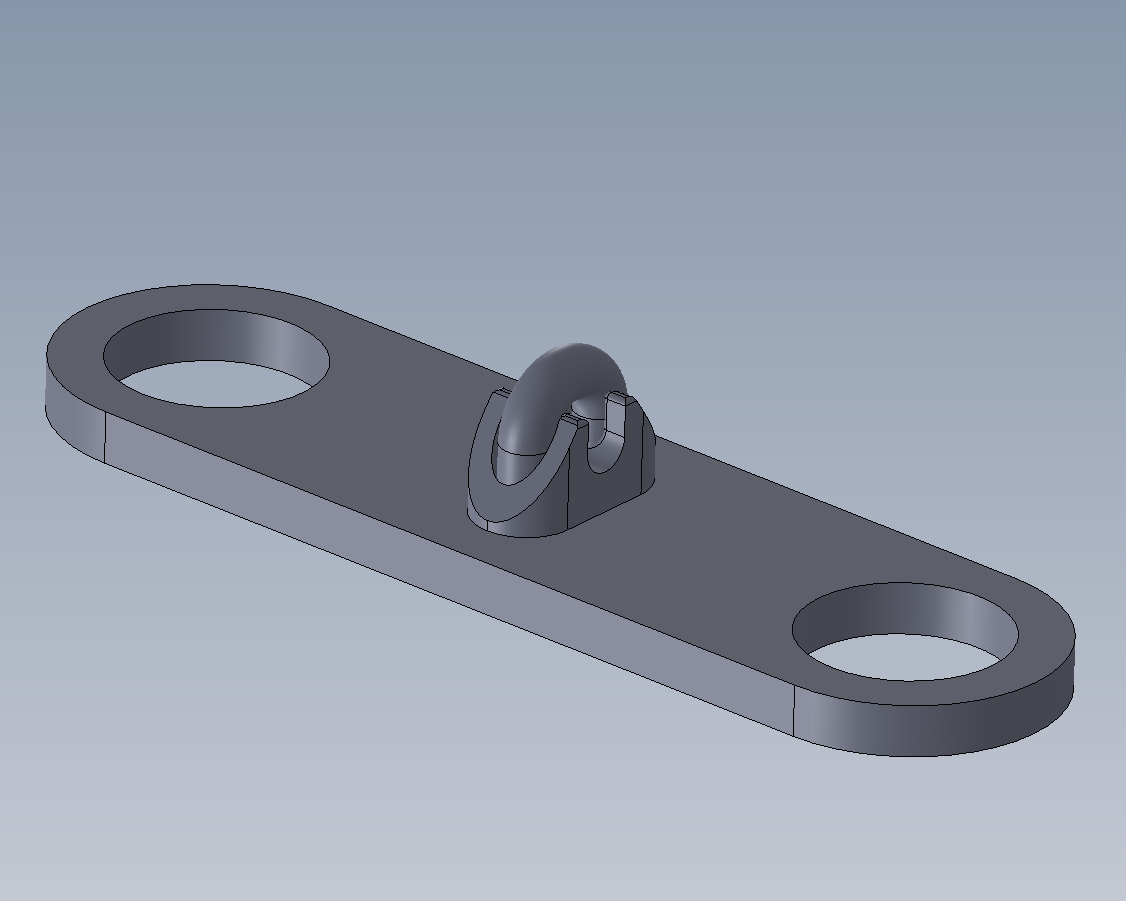
\includegraphics[width=\linewidth]{figures/guy_grounding_asembly[1].png}
        \caption{Guy Grounding Assembly}
    \end{minipage}
    \hfill
    \begin{minipage}[t]{0.48\textwidth}
        \centering
        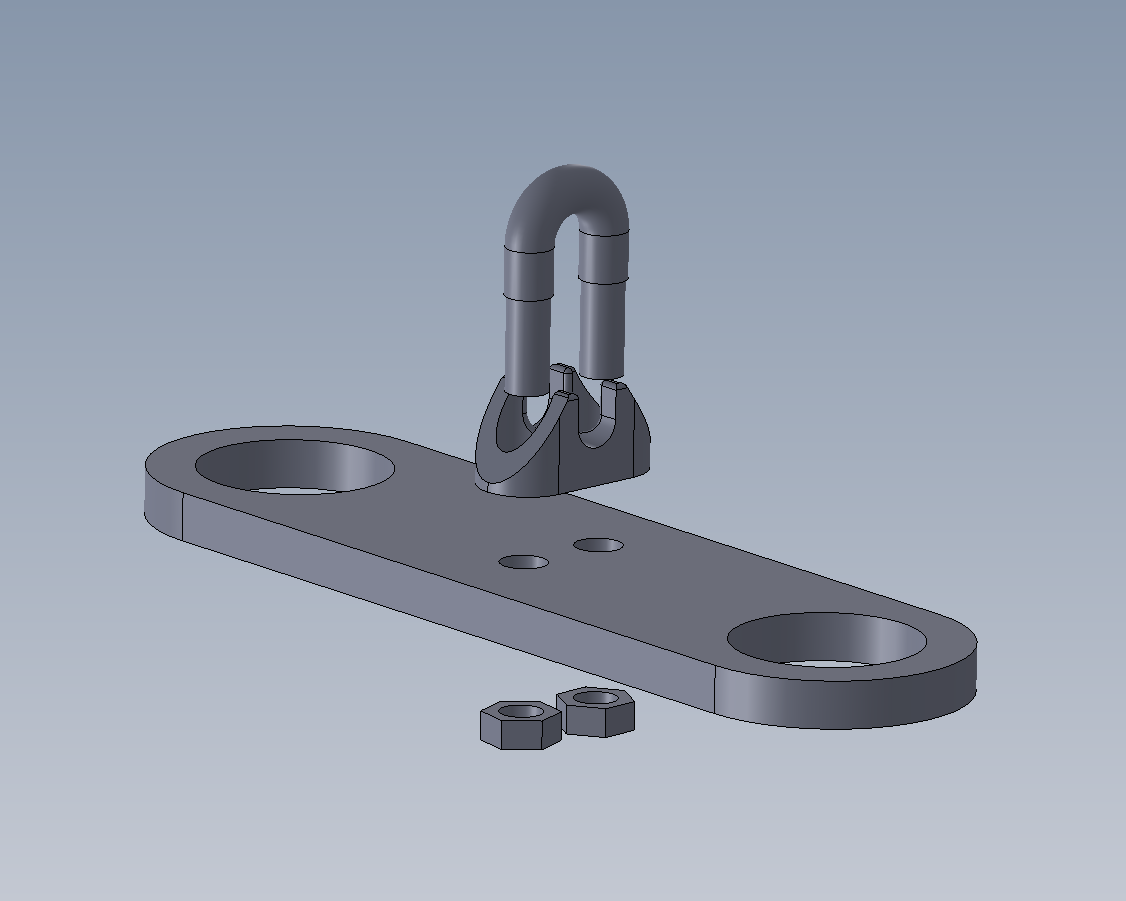
\includegraphics[width=\linewidth]{figures/guy_grounding_asembly_exploded[1].png}
        \caption{Guy Grounding Assembly Exploded}
    \end{minipage}
\end{figure}
These grounding is then anchored into the ice by 2 M20 anchor rods. (Covered in detail in section 2.5.2). They will be anchored at a radial distance from the central mast of 3 m and evenly spaced such that the guy ropes are aligned with the corners of the housing cube. The long sides of the grounding plates will be aligned with the direction of the guy ropes.

\begin{figure}[H]
    \centering
    \begin{minipage}[t]{0.48\textwidth}
        \centering
        \includegraphics[width=\linewidth]{figures/final build views.PNG}
        \caption{Final Build Views}
    \end{minipage}
\end{figure}



\subsection{Cost Optimisation}
Cost optimisation was a major design consideration particularly given the economic constraints that were defined in the project’s `User Requirements Specification'. The total system cost has to remain sufficiently low in order to ensure that the renewable energy system would provide meaningful cost savings when compared with the diesel fuel consumption at the EastGRIP research camp.

This entailed the implementation of several meaningful strategies to cut down manufacturing cost.

First of all, the design is mostly composed of commercial off-the-shelf components wherever possible. The wind turbine, telescopic mast, solar panels, sensors and battery system are all products that are commercially available and are integrated directly into the overall system architecture. By using these pre-manufactured components, the need for complex custom manufacturing is completely eliminated and reduces drastically production costs and development time.

Material selection was also of major importance for cost optimisation. By choosing HSLA structural steel for the structural housing, a good balance between mechanical performance, weight and material cost was obtained. In addition, HSLA structural steel offers quite good corrosion resistance which therefore reduces the need for expensive protective coatings or any additional treatments.

Another consideration during the design process was the optimisation of logistical costs. Because the system needs to be transported to the EastGRIP research site by aircraft, the whole structure was designed to be modular and easily disassembled, which allows the components to be packed neatly and efficiently within the aircraft pallet constraints. The main objective was to limit the whole structure to no more than one pallet as anything more would increase the overall transportation costs and also increase the risk of damaging the design.

Overall, these design choices ensure that the system remains economically feasible while still meeting all the structural and operational requirements to be deployed in Arctic environments.

\subsection{Component Standardisation}
Standardisation was incorporated throughout the design process as it was an efficient way to simplify both manufacturing and long-term maintenance. Whenever possible, the structural components were designed to use repeated geometries and standardised mounting interfaces.

For example, the long and short housing side plates have similar hole patterns and fastening arrangements. This technique allows for identical machining operations to be used during manufacturing which reduces production complexity and improves the consistency between the various components.

In a similar fashion, the structural frame uses repeated 90° angle brackets and identical fastener sizes wherever possible. By standardising the fasteners, the number of different required tools are reduced.

Electrical components were also selected with standardisation in mind. The environmental sensors, microcontroller and data logging system all use widely available connectors and wiring standards which allows the electrical system to be assembled easily and only using commercially available cables and connectors.

This also improves the long-term reliability of the system as any component that needs to be replaced during operation. It is much easier to replace a standardised part than a specialised custom component.

Overall, the design prioritises simplicity, modularity and standardisation. This ensures that the system can be manufactured efficiently but still remain robust enough to be deployed in extreme conditions.

%--------------------------------------------------
\section{Design for Sustainability - SO}

The overarching goal of this project was to research, design, and develop a device that provides sustainable power for a small camp in Arctic conditions. All power produced and consumed within this device is sustainable from the solar panels and wind turbine in order to provide an alternative source of energy as the majority of camps in remote regions will tend toward using diesel generators. We attempted to alleviate this issue by reducing the fuel consumption in remote Arctic camps; with our target location being EastGRIP in central Greenland. 

We do not believe the manufacturing of this product can be adjusted to accomodate recycled or plan-based materials besides potentially recycled aluminium in the base design. The greatest issue stems from the necessity to purchase a large portion of the components within the design, specifically: the turbine, solar panels, circuit components and sensors. Recycled copper wiring may also be possible, but this would provide an insignificant improvement.

Ultimately, it is important to acknowledge that our product will have a significant predicted lifetime - potentially in excess of 15 years - while producing sustainable, renewable energy throughout this period. It will allow for a reduction in burning fossil fuels that are the main alternative in this market, hence intending to save costs over this lifespan.


%--------------------------------------------------
\section{Commercial Considerations -- CJ}

\subsection{Cost Analysis}

The total predicted capital cost of the proposed hybrid renewable system is
approximately £9{,}209, with an estimated uncertainty of $\pm 5\%$ to account
for fluctuations in component and procurement prices. The system is expected
to generate approximately $2{,}850\,\text{kWh}$ of electricity during the
summer operating season, primarily from solar power with a smaller
contribution from wind. As electricity at the EastGRIP camp is currently
supplied by diesel generators, this renewable generation directly displaces
diesel fuel consumption and therefore reduces the operational cost of power
supply.

To estimate the equivalent diesel displacement, the energy content of diesel
and typical generator efficiencies were considered. Diesel contains
approximately $137{,}381\,\text{Btu}$ per US gallon, while
$1\,\text{kWh} = 3{,}412\,\text{Btu}$. The thermal energy content of diesel is
therefore

\begin{equation}
E_{\text{diesel}}=
\frac{137{,}381}{3{,}412}
\approx 40.26 \;\text{kWh}_{\text{th}} \text{ per gallon}.
\end{equation}

For a diesel generator with electrical efficiency $\eta$, the electrical
energy produced per gallon of diesel is

\begin{equation}
E_{\text{elec}} = 40.26\,\eta \;\text{kWh per gallon}.
\end{equation}

The equivalent diesel displacement associated with the additional renewable
generation is therefore

\begin{equation}
\text{Diesel saved} = \frac{E}{40.26\,\eta},
\end{equation}

where $E$ is the electrical energy generated. Using
$E = 2{,}850\,\text{kWh}$ and a realistic generator efficiency range of
$\eta = 0.25$--$0.40$, the proposed system is estimated to displace
approximately $177$--$283$ US gallons of diesel per season, equivalent to
approximately $670$--$1{,}072$ litres of fuel.

Table~\ref{tab:diesel_displacement_updated} summarises the diesel
displacement over the assumed efficiency range.

\begin{table}[h]
\centering
\caption{Estimated diesel displacement from $2{,}850\,\text{kWh}$ seasonal renewable generation}
\label{tab:diesel_displacement_updated}
\begin{tabular}{ccc}
\toprule
Generator efficiency $\eta$ & Electrical output (kWh/gal) & Diesel displaced (US gal) \\
\midrule
0.25 & 10.07 & 283 \\
0.30 & 12.08 & 236 \\
0.35 & 14.09 & 202 \\
0.40 & 16.10 & 177 \\
\bottomrule
\end{tabular}
\end{table}

The commercial value of this displaced fuel depends primarily on the
delivered cost of diesel at remote inland camps, where logistics,
transport, and storage dominate the overall energy cost. Assuming a
representative delivered fuel cost of \$33 per gallon and a generator
efficiency of $\eta = 0.30$, the system displaces approximately
$236$ gallons of diesel per season, giving an estimated seasonal saving of

\begin{equation}
236 \times 33 \approx \$7{,}788
\end{equation}

or approximately £5{,}800 per season.

To illustrate the sensitivity of savings to both fuel price and generator
efficiency, Table~\ref{tab:savings_sensitivity_updated} presents the
estimated seasonal savings across a realistic range of assumptions based on a
\$33 per gallon delivered-fuel benchmark with $\pm 20\%$ variation.

\begin{table}[h]
\centering
\caption{Estimated seasonal savings for $2{,}850\,\text{kWh}$ renewable generation}
\label{tab:savings_sensitivity_updated}
\begin{tabular}{cccc}
\toprule
Generator efficiency $\eta$ & Savings @ \$26.4/gal & Savings @ \$33/gal & Savings @ \$39.6/gal \\
\midrule
0.25 & \$7{,}475 & \$9{,}344 & \$11{,}213 \\
0.30 & \$6{,}230 & \$7{,}787 & \$9{,}344 \\
0.35 & \$5{,}340 & \$6{,}674 & \$8{,}009 \\
0.40 & \$4{,}672 & \$5{,}840 & \$7{,}008 \\
\bottomrule
\end{tabular}
\end{table}

Using the broader delivered-fuel range discussed in the supporting analysis,
seasonal savings are estimated to lie between approximately
\$5{,}840 and \$12{,}742 per season, equivalent to approximately
£4{,}350--£9{,}490. This demonstrates that the commercial attractiveness of
the design is strongly linked to the true marginal cost of diesel delivery to
the site rather than the nominal retail price of fuel.

The simple payback period may therefore be estimated from

\begin{equation}
\text{Payback period} =
\frac{\text{Capital cost}}{\text{Seasonal savings}}.
\end{equation}

Using the base-case seasonal saving of approximately £5{,}800, the simple
payback period is

\begin{equation}
\text{Payback period} =
\frac{9{,}209}{5{,}800}
\approx 1.6 \;\text{seasons}.
\end{equation}

A conservative case may be obtained by assuming a delivered fuel valuation of
\$26.4 per gallon, a higher generator efficiency of $\eta=0.40$, and only
$80\%$ of the generated electricity directly displacing diesel operation.
Under these assumptions, seasonal savings are approximately £2{,}785,
corresponding to a payback period of approximately $3.3$ seasons. By
contrast, an optimistic case using \$45 per gallon delivered fuel cost,
$\eta=0.25$, and full diesel displacement gives seasonal savings of
approximately £9{,}490 and a payback period of approximately one operating
season. Applying the stated $\pm 5\%$ capital-cost uncertainty gives a
base-case payback range of approximately $1.5$--$1.7$ seasons, which remains
commercially attractive for a remote polar installation.

\subsection{Market Viability}

The proposed system is commercially viable because it addresses a highly
specialised but high-value engineering problem: reliable electricity
generation at remote polar research camps where power is currently supplied
by diesel generators. In such environments, the economic burden arises not
only from fuel purchase but also from transport, handling, storage and
resupply risk. The proposed hybrid solar--wind system therefore offers value
through both direct fuel savings and reduced dependence on complex logistics.
Although the target market is niche, organisations operating remote
scientific, monitoring or expeditionary facilities are likely to value
technologies that reduce fuel demand, improve sustainability credentials and
increase energy resilience. Marketing expenditure would therefore be modest
and focused on institutional procurement routes, technical demonstrations and
specialist research or polar operations conferences rather than mass-market
advertising.

\subsection{Product Lifecycle}

The overall system is expected to remain commercially viable for
approximately $10$--$15$ years before major refurbishment or replacement is
required. Structural components such as the support frame, tower and mounting
hardware are expected to have the longest service life, whereas electrical
subsystems such as charge control equipment, batteries and power-conditioning
components are more likely to require replacement on a shorter timescale.
This lifecycle is sufficient to recover the initial capital cost within the
early years of operation and then provide several further seasons of net
operational savings before major reinvestment is necessary.

\subsection{Expected Sales}

Expected sales volume is limited by the specialist application of the design.
This is not a consumer product and should not be presented as such. A
realistic target market would consist of remote polar research stations and
similar off-grid scientific installations where diesel logistics remain a
major operational burden. On this basis, a conservative estimate would be the
sale of approximately $5$--$15$ systems over the product lifecycle,
depending on institutional uptake, available funding, and site-specific
energy demand. While this sales volume is low compared with mainstream energy
products, the high operational value of each installation supports the
commercial rationale for development.

\subsection{Maintenance and Warranties}

To minimise operational disruption, the system should be designed around
modular components that can be inspected and replaced individually. Routine
maintenance would consist of seasonal inspection of the turbine, solar array,
electrical connections, mounting points and protective housings, with
replacement of wear-prone components where necessary. This is particularly
important in remote environments where repair opportunities are limited and
system downtime carries disproportionate operational cost. A warranty period
of $3$--$5$ years would be appropriate for electrical components, while
structural elements could be covered over a longer design life subject to
correct installation and regular inspection. This arrangement provides a
realistic balance between commercial responsibility and the operational risks
associated with deployment in extreme environments.


%--------------------------------------------------
\section{Code of Practice and Standards - CJ}

\subsection{Applicable Engineering Standards}

\begin{table}[H]
\centering
\caption{Relevant engineering standards considered during the design process}
\begin{tabular}{l l p{9cm}}
\hline
Standard & Domain & Relevance to Design \\
\hline
BS 7671 & Electrical installations & Safe low-voltage DC wiring and battery integration \\
IEC 60364 & Low-voltage electrical systems & General electrical installation principles \\
IEC 61400 & Wind turbine systems & Safety and operational standards for small wind turbines \\
IEC 61215 & Photovoltaic modules & Performance and durability certification for the Trina 440 W photovoltaic modules used in the system \\
IEC 61730 & Photovoltaic safety & Electrical safety of PV modules \\
BS 8888 & Engineering drawings & Standardised manufacturing documentation \\
ISO 12100 & Machinery safety & Machinery safety risk assessment for assembly and seasonal deployment \\
\hline
\end{tabular}
\end{table}
These standards are particularly relevant for the EastGRIP deployment environment, where low temperatures, seasonal assembly and limited maintenance access place additional reliability requirements on the system.

\subsection{Professional Codes of Conduct}
Professional practice during the design process was guided by recognised engineering codes of conduct, particularly the Engineering Council’s \textbf{UK-SPEC} framework and the \textbf{Institution of Engineering and Technology (IET) Code of Conduct}. These frameworks emphasise the responsibility of engineers to prioritise safety, environmental stewardship and technical integrity throughout the design lifecycle. In the context of the proposed renewable power system, due diligence was applied in the selection of commercially certified components (e.g. wind turbine and photovoltaic modules), conservative electrical system design using a 12\,V architecture, and the incorporation of structural stability measures such as guy-wire supports. Particular consideration was given to reliability and safe operation within the remote Arctic environment of the EastGRIP research station, where maintenance opportunities are limited and system failure could disrupt scientific operations.

\subsection{Avoiding Stakeholder Misinterpretation}
Potential misinterpretation of system capabilities by stakeholders has also been considered during the design process. As the system is intended to be deployed and assembled by general research staff rather than specialist engineers, clear documentation and straightforward mechanical assembly have been prioritised. For example, the modular structural frame utilises standardised fasteners and clearly defined mounting components to minimise assembly errors during seasonal installation. Additionally, renewable power systems inherently produce variable outputs due to fluctuating wind and solar conditions. Non-technical stakeholders may therefore incorrectly assume continuous power availability. To mitigate this risk, system documentation specifies expected seasonal energy production (approximately 2,800\,kWh), operational limits and the requirement for inspection and verification during each seasonal reassembly of the system.


%--------------------------------------------------
\section{Discussion} %- SAM + NICO - STILL NEED TO EVALUATE URS
Overall, the proposed hybrid wind–solar system satisfies the primary URS constraints relating to portability, environmental operation, and minimum power production, while offering a significant reduction in fuel dependency compared with conventional diesel-based power solutions.

\subsection{Evaluation of future Turbine Implementation - NW}
The main competitor to our device is diesel generators due to the inaccessibility of typical power infrastructure and the fact that research of sustainable power generation in remote Arctic environments is still ongoing. This provides a significant gap in the market for our project, however, it is very important to acknowledge that our current power projections indicate that this device will not be capable of powering a camp on its own. The money saved from not needing to repeatedly purchase fuel does provide a noticeable benefit for our customers but there will always be an inherent unreliability in power produced from wind and solar power.

An objective of the project is to evaluate the feasibility of the design outlined for potential deployment in similar locations. It is important to consider that other sites may have slightly different power demands depending on how energy is produced locally. This is likely because other locations may not experience the same extended daylight hours available at the EastGRIP camp and may therefore require a larger contribution from wind power.

To investigate this possibility, safety calculations were carried out for several alternative wind turbine options using the same methodology applied to the RYSE AIR 30 turbine, while assuming similar wind conditions.

Table~\ref{tab:alt_turbines} summarises the safety factors obtained for alternative turbine options when used with the proposed support structure. The safety factors are calculated relative to the RYSE AIR 30 turbine, which has a rated power of $0.4\,\mathrm{kW}$.

\begin{table}[H]
\centering
\caption{Safety factors for alternative wind turbine options}
\label{tab:alt_turbines}
\begin{tabular}{>{\raggedright\arraybackslash}p{4cm} c c c c}
\hline
Alternative turbine & Rated Power & Swept Diameter & Guy Rope FoS & Ground Anchor FoS \\
\hline
Rutland WG1200 & 1 kW & 1.22 m & 32.0 & 73.6 \\
Bornay Wind 3000 & 3 kW & 4 m & 5.7 & 13.2 \\
Bergey Excel 5 & 5 kW & 6.2 m & 2.5 & 5.8 \\
\hline
\end{tabular}
\end{table}

\subsection{Evaluation Against Design Specifications - SO}
The proposed system significantly exceeds the URS power target and is therefore likely to be a suitable solution for Arctic research camps operating under conditions similar to those at EastGRIP. As both the solar panels and wind turbine are capable of operating in warmer environments, the design is also potentially applicable to other remote locations with similar infrastructure constraints.

The weight of the whole system is significantly lighter than the 3 tonne maximum while simultaneously fitting on the aircraft pallet and being below the maximum operating height. This device undoubtedly beats the performance target of 1.7kWh/day and maintains functionality even in the worst expected conditions of 40 kt wind speeds and at \(-\SI{30}{\celsius}\). An internal temperature of \SI{0}{\celsius} will be maintained consistently using both insulation and a silicone pad heater that reaches a peak power use of 22W.

The predicted final cost of the system is expected to be $\approx \pounds9200$ which is comfortably within our maximum price.
The URS has also been updated to accomodate the Must that the device should be producing a minimum power at any time which has been resolved. 

\subsection{Performance Limitations and System Uncertainty - SO}
The greatest uncertainties in our predictions stems from the unpredictability of weather, as a strong storm that lasts a long time may prevent both the solar panels and turbine from producing power in that time frame. Although prolonged storms are unlikely, extended periods of low solar irradiance combined with low wind speeds could temporarily reduce power production. There will always be an inherent unreliability in power produced from wind and solar power.

\subsection{Opportunities for Design Improvement - SO}
The relative contribution of wind generation compared to the solar panels was lower than initially anticipated.

If the transport and setup capabilities at a deployment site allow for handling a larger turbine, the same system architecture could potentially be implemented using a higher rated wind turbine.

Of the additional requirements outlined in the URS, all sensors are capable of recording data at higher sampling frequencies to support improved analysis. However, the data must currently be accessed manually by removing the SD card from the electrical enclosure. As a result, data retrieval will realistically occur monthly. Implementing remote telemetry or wireless data transfer would therefore represent a valuable future enhancement to the system.

\subsection{Implications of Material and Technology Choices - SO}
Turbine de-icing is also addressed using a new composite coating for the blades which should result in near zero ice accretion.
\\
\\
Overall, the analysis demonstrates that the proposed hybrid renewable power system is technically feasible for Arctic deployment and satisfies the primary URS constraints, while also providing clear opportunities for performance improvement through increased turbine capacity and enhanced data telemetry.

%--------------------------------------------------
\section{Conclusion - SO, IK}

In summary, this project has successfully delivered a reliable, high-performing, and sustainable remote power generation device, That also logs environmental data, well-suited for deployment in demanding Arctic environments. The key outcomes of this project are as follows:

\begin{itemize}
    \item The device is projected to generate \textbf{2800~kWh} per Arctic summer deployment, with demonstrated resilience to wind speeds up to 40~kt and temperatures as low as $-30^\circ$C.
    \item A \textbf{93/7 solar-to-wind power split} ensures consistent energy generation across varying environmental conditions, including periods of reduced solar availability.
    \item Complete \textbf{autonomous environmental data logging system (EDLS)} integrates four environmental parameters: solar irradiation, ambient temperature, local wind speed and direction. This system independently operates within the electrical enclosure powered by the battery and autonomously stores data. 
    \item Integrated \textbf{thermal management and moisture control} systems protect internal components, significantly reducing the likelihood of electrical or structural failure within the device's operational lifecycle.
    \item The device presents a \textbf{commercially viable alternative to diesel generation}, reducing the logistical burden of continuous fuel resupply while requiring only periodic maintenance.
    \item The device would \textbf{not fully replace diesel generation in larger camps} but introduces significant relief from the burden of power supply of a typical fossil fuel generator.
    \item The product is expected to cost roughly $\approx \pounds 9200$ giving an ROI in 1 - 2 years after purchase.
    \item It has an expected lifespan of 15 years with only limited maintenance needed on site. The main risks associated with its construction and implementation are associated with rusting or wearing of turbine components.
\end{itemize}

Future iterations of this device would benefit from an upgraded turbine, an expanded battery capacity, and broader environmental testing to validate performance beyond Arctic applications. Overall, this project has demonstrated strong technical and commercial foundations, with clear potential for scalable deployment across remote regions where sustainable off-grid power is critically needed.

%----------------------------------------
\section{Project Planning - CJ}

\subsection{Management Approach}

Project coordination was maintained through structured biweekly meetings held on Tuesdays and Fridays, supplemented by continuous communication via Microsoft Teams and Messenger. Tuesday meetings focused on reviewing progress against planned tasks, resolving technical uncertainties, and defining objectives for the upcoming work period. Friday meetings acted as formal checkpoints to assess task completion, identify deviations from the schedule, and reallocate resources where necessary. An example of one of the Friday meetings is provided in Appendix~H.

The project timeline was initially developed to structure activities across three phases. Phase 1 (Michaelmas Term) focused on feasibility analysis and culminated in the feasibility report submission. Phases 2 and 3, undertaken during Epiphany Term, encompassed detailed design, system integration, and final report development.

The Gantt chart in Figure~\ref{fig:Gantt} presents the schedule for Phases 2 and 3. Detailed design activities, including calculations, component selection, and CAD modelling, were prioritised early in the schedule and executed in parallel to reduce overall project duration. System integration was dependent on the completion of core design elements, while report development was initiated prior to design freeze to mitigate time constraints approaching the submission deadline.

Key project milestones included the design freeze, final presentation, and report submission. These milestones served as decision gates to ensure the design remained on schedule and met required specifications. The original project timeline from Phase 1, is provided in Appendix~I.
\subsection{Team Contributions}

Task allocation was structured according to project phases to ensure efficient use of team expertise and balanced workload distribution. Responsibilities were assigned based on technical strengths while maintaining collaboration across interconnected tasks.

\begin{table}[H]
\centering
\caption{Summary of team contributions by project phase}
\begin{tabular}{lll}
\toprule
\textbf{Phase} & \textbf{Task} & \textbf{Responsible Member(s)} \\
\midrule
Concept \& Planning & Stakeholder analysis, system definition, URS & CJ, TB \\
Concept \& Planning & Component Compatibility Considerations & NW\\
Concept \& Planning & Battery System Evaluations & NW \\
Concept \& Planning & Local Solar Resource & IK \\
Concept \& Planning & Environmental Sensors Evaluation & IK \\
Design Development & Concept Refinement and Evaluation & TB \\
Design Development & Structural configuration and Final dimension Estimation & TB \\
Detailed Design & Solar Energy Generation & IK \\
Detailed Design & Environmental data logging System & IK \\

Detailed Design & Wind turbine and anti-icing system & OM \\
Detailed Design & Justification for Wind Turbine & OM \\
Detailed Design & Circuit safety and insulation design & SO \\
Detailed Design & CAD modelling and mechanical integration & NW, TB \\
Detailed Design & Structural Calculations & NW \\
Design for manufacture & Production volume and Manufacturing Methods & TB \\
Design for manufacture & Tooling and Assembly analysis & TB \\
Design for manufacture & Cost optimisation and standardisation & TB \\
System Integration & Sensor logic and system integration & CJ \\
Commercial Analysis & Cost evaluation and feasibility & CJ \\
Commercial Analysis & Code of Practice and Standards & CJ \\
Documentation & Executive summary, conclusion, discussion & OM, SO, IK \\
Documentation & LaTeX formatting, grammar and report integration & CJ, SO, IK, TB\\
\bottomrule
\end{tabular}
\end{table}

While primary responsibilities were defined, collaboration occurred across all phases, particularly during integration and report development, ensuring consistency and technical coherence throughout the design.


\begin{landscape}

\begin{figure}[p]
\centering

\begin{ganttchart}[
    time slot format=isodate,
    x unit=0.3cm,
    y unit chart=0.7cm,
    bar height=0.6,
    group height=0.7,
    milestone height=0.6,
    vgrid,
    hgrid
]{2026-01-13}{2026-03-21}

\gantttitlecalendar{year, month=name, week} \\

% Phase 1
\ganttbar{Feasibility Report Corrections}{2026-01-13}{2026-01-20} \\

% Phase 2
\ganttgroup{Detailed Design}{2026-01-20}{2026-03-10} \\
\ganttbar{Component selection}{2026-01-20}{2026-02-10} \\
\ganttbar{Sensors Analysis}{2026-01-20}{2026-01-27} \\
\ganttbar{Ice Accretion Analysis}{2026-01-20}{2026-01-27} \\
\ganttbar{Sensor/Circuitry Design}{2026-01-27}{2026-02-03} \\
\ganttbar{CAD modelling}{2026-01-27}{2026-02-17} \\
\ganttbar{Sensor Logic Diagrams}{2026-01-27}{2026-02-10} \\
\ganttbar{Subsystem integration}{2026-02-10}{2026-03-06} \\
\ganttbar{Creating Presentation}{2026-02-17}{2026-02-20} \\
\ganttbar{Presentation rehearsal}{2026-02-20}{2026-02-23} \\
\ganttmilestone{Presentation}{2026-02-23} \\

% Phase 3
\ganttgroup{Design Report Portfolio}{2026-02-24}{2026-03-19} \\
\ganttbar{Finalize Calculations}{2026-02-24}{2026-03-6} \\
\ganttbar{Research into Report content}{2026-02-28}{2026-03-10} \\
\ganttmilestone{Design freeze}{2026-03-10} \\
\ganttbar{Final write up}{2026-03-11}{2026-03-17} \\
\ganttbar{Latex formatting \& Submission}{2026-03-17}{2026-03-19} \\
\ganttmilestone{Final report submitted}{2026-03-19}

\end{ganttchart}
\caption{Project schedule from feasibility report submission to final design report deadline}
    \label{fig:Gantt}
\end{figure}
\end{landscape}

\subsection{Reflection on Execution}
The planned project schedule was largely adhered to, with the Gantt chart accurately reflecting progress throughout Phases 2 and 3. Minor deviations occurred during the sensor integration stage, where initial design assumptions regarding blade-mounted sensors were found to be impractical. This required additional investigation into alternative approaches, leading to the adoption of a super-hydrophobic coating solution. As this modification did not require significant changes to the electrical system, its impact on the overall timeline was minimal.

Variability in team experience with LaTeX formatting presented a potential bottleneck during the documentation phase. This risk was mitigated through redistribution of formatting responsibilities to a single team member, allowing other members to focus on technical content generation. This ensured efficient report compilation without delaying submission.

Overall, the project demonstrated effective planning, communication, and adaptability. Parallel task execution and structured review points enabled the team to maintain progress despite minor technical challenges, resulting in timely completion of all deliverables.

%--------------------------------------------
\begin{thebibliography}{99}

\bibitem{Weight} \url{https://www.constructionequipmentguide.com/charts/crawler-loaders/caterpillar/955l/3122#:~:text=The%20Caterpillar%20955L%20Crawler%20Loader,breakout%20force%20of%2022%2C930%20lbs.}

\bibitem{Packed Dimensions} \url{https://www.aclairshop.com/463L_air_cargo_pallet.php}

\bibitem{Power Production} \url{https://icedrill.org/sites/default/files/NEEM2010FieldPlan.pdf https://eastgrip.nbi.ku.dk/documentation/2022/egrip2022fieldplan_1stversion.pdf}

\bibitem{Weather} \url{https://eastgrip.nbi.ku.dk/documentation/2022/egrip2022fieldplan_1stversion.pdf}

\bibitem{Internal Heating} \url{https://eastgrip.nbi.ku.dk/documentation/2022/egrip2022fieldplan_1stversion.pdf}

\bibitem{Fuel usage}\url{https://www.165aw.ang.af.mil/News/Article-Display/Article/1271932/109th-aw-finishes-up-fifth-rotation-in-greenland/}

\bibitem {Fuel Price} \url{https://gasprices.aaa.com/state-gas-price-averages/}

\bibitem{Battery Final} \url{https://sabik.com/wp-content/uploads/2024/10/sabik_marine_datasheet_saft_sunnicd_batteries_20201.pdf}

%SOLAR REFERENCES 
\bibitem{eastgrip}
EastGRIP Ice Core Project, “Contact,” Available: \url{https://eastgrip.nbi.ku.dk/contact/}

\bibitem{dydqi}
DQYDJ, “Daylight Hours Calculator,” Available: \url{https://dqydj.com/daylight-hours-graph/}

\bibitem{trina}
Trina Solar, “Vertex S+ NEG9RC.27 Photovoltaic Module Datasheet,” 2023. Available: \url{https://static.trinasolar.com/sites/default/files/VertexS_NEG9RC.27_EN_2023_B_web.pdf}

\bibitem{pvgis}
European Commission Joint Research Centre (JRC), “PVGIS – Photovoltaic Geographical Information System,” Available: \url{https://re.jrc.ec.europa.eu/pvg_tools/en/}

\bibitem{ice}
R. Frederking, O. J. Svec, and G. W. Timco, “On measuring the shear strength of ice,” in \textit{IAHR Ice Symposium}, Sapporo, vol. 3, pp. 76–98, 1988.

\bibitem{ECO-WORTHY Mounting Bracket}
ECO-WORTHY Mounting Bracket Available: \url{https://www.eco-worthy.com/products/updated-adjustable-multi-piece-solar-panel-mounting-brackets-for-1-4-pieces-of-solar-panels?srsltid=AfmBOorzyl6pK08xs0c_RcyA0t_SVE6kvGIk0hP1EYbvIQlQL4ZujqiB}



\bibitem{Pole}
Mast: \url{https://www.clarkmasts.com/media/dyn-docs/products/ptsl-m-e-cms-10112014.pdf}

\bibitem{fasteners}
Off the shelf components: \url{https://www.f-e-s.co.uk/m18-hexagon-full-nuts-stainless-steel-a2-304-din-934.html?}

\bibitem{Cables}
Cables:\url{https://www.norfolkmarine.co.uk/wire-rope-5mm-1-x-19-stainless-steel-316?}
%ELECTRICAL COMPINENTS REFERENCES

\bibitem{pyranometer}
Kipp \& Zonen, 
\textit{CMP3 Pyranometer}. 
[Online]. Available: https://www.kippzonen.com/Product/11/CMP3-Pyranometer


\bibitem{ampbox}
Kipp \& Zonen, 
\textit{AMPBOX Signal Amplifier}. 
[Online]. Available: https://www.kippzonen.com/Product/37/AMPBOX-Amplifier

\bibitem{windsensor}
Gill Instruments Ltd., 
\textit{WindSonic 75 Ultrasonic Anemometer Datasheet}. 
[Online]. Available: https://www.omniinstruments.co.uk/wp-content/uploads/2024/02/WindSonic-75-Ultrasonic-Anemometer.pdf

\bibitem{rs232}
AYMBH, 
\textit{MAX3232 RS232 to TTL Serial Port Converter Module}. 
Amazon UK. [Online]. Available: https://www.amazon.co.uk/AYMBH-MAX3232-Serial-Converter-Transceiver/dp/B0DKR34X7P

\bibitem{tempsensor}
AZ-Delivery, 
\textit{DS18B20 Waterproof Temperature Sensor}. 
[Online]. Available: https://www.az-delivery.uk/products/2xds18b20wasserdicht




\bibitem{dcdc}
TDK Corporation, 
\textit{i7C4W012A050V DC–DC Converter}. 
[Online]. Available: https://product.tdk.com/en/search/power/switching-power/dc-dc-converter/info?part\_no=i7C4W012A050V-002-R


\bibitem{arduino}
Arduino, 
\textit{Arduino Uno Rev3}. 
[Online]. Available: https://uk.webuy.com/product-detail/?id=SDESARDUNLREV3B



\bibitem{sdmodule}
DFRobot, 
\textit{Micro SD Card Module for Arduino Uno/Mega}. 
[Online]. Available: https://uk.farnell.com/dfrobot/dfr0229/micro-sd-module-arduino-uno-mega/dp/3769941


\bibitem{sdcard}
Kingston Technology, 
\textit{Industrial SD Card Datasheet}. 
[Online]. Available: https://www.kingston.com/datasheets/SDCIT2\_en.pdf


\bibitem{heater}
RS Components, 
\textit{Silicone Rubber Heater Datasheet}. 
[Online]. Available: https://docs.rs-online.com/794f/A700000007920404.pdf




\bibitem{thermostat}
Aideepen, 
\textit{Digital Temperature Controller Thermostat}. 
Amazon UK. [Online]. Available: https://www.amazon.co.uk/Aideepen-Thermostat-Temperature-Controller-Thermometer/dp/B08DD9LNZL



\bibitem{enclosure}
https://www.amazon.co.uk/LEPEVNEY-IP65-ABS-Waterproof-Junction/dp/B0CR3TW2DK







\bibitem{adfreeze}
Adfreeze strength of model piles in ice
\url{https://nrc-publications.canada.ca/eng/view/ft/?id=058a0f1f-1040-477b-ad1e-717472daebf2}

% OLLIE
\bibitem{antiicingstudy}
Preparation and Anti-Icing of Hydrophobic Polypyrrole Coatings on Wind Turbine Blade 
https://pdfs.semanticscholar.org/ecaa/4cfa5437032f52f214e64a8452153353fcd9.pdf

\bibitem{PPy}
https://www.scientificlabs.co.uk/product/organic-and-printed-electronics/577030-25G

\bibitem{PVDF Powder}
https://www.scientificlabs.co.uk/product/hydrophobic-polymers/182702-100G

\bibitem{NMP Solvent}
https://www.sigmaaldrich.com/GB/en/product/sial/328634
\bibitem{Carbon Steel}
\url{https://www.chinasteelmarket.com/prices/html/Boiler-Steel-Plate-Prices-in-China-on-January-9_30371.html}
\bibitem{orbital fasteners}
Orbital Fasteners, 
\textit{M18 Hexagon Bolts (DIN 931) Product Listings}. 
Available at: \url{https://www.orbitalfasteners.co.uk} 
(Accessed: 2026).

\bibitem{accu components}
Accu Components, 
\textit{Metric Fasteners and Precision Components Catalogue}. 
Available at: \url{https://www.accu.co.uk} 
(Accessed: 2026).

\bibitem{rs components}
RS Components Ltd., 
\textit{Engineering Components and Fasteners Catalogue}. 
Available at: \url{https://uk.rs-online.com} 

\bibitem{usermanual}
https://cdn.shopify.com/s/files/1/0849/0362/5052/files/AIR_Wind_Turbines_User_Manual_JAN24.pdf?v=1733501874

\bibitem{windpowerestimation}
https://cdn.standards.iteh.ai/samples/12543/d5d66c679e54480bb7469ebdb84ddd29/IEC-61400-12-1-2005.pdf

\bibitem{windturbine}
https://www.ecopowershop.com/products/air-30-wind-turbine-off-grid-12v-small

\end{thebibliography}


%==================================================
% APPENDICES
%==================================================
\section{Appendix} - INDIVIDUALLY 
\appendix



\section{Adjusted panel tilt derivation}
\label{app:Adjusted panel tilt derivation}

EastGRIP site:
\[
75.63248^\circ \text{N}, \quad 35.98911^\circ \text{W}
\]
Conventional tilt heuristic:
\[
\theta \approx \text{Latitude} + \phi_{\text{season}}
\]
\[
\phi_{\text{season}} = -15^\circ \quad (\text{summer})
\]
\[
\text{Tilt} \approx 60^\circ
\]
Adjustment applied:
\[
\phi_{\text{adj}} = -10^\circ
\]
Adjusted tilt:
\[
\text{Tilt}_{\text{adj}} \approx \text{Latitude} + \phi_{\text{season}} + \phi_{\text{adj}} = 50^\circ
\]
Projected area reduction:
\[
A_{\text{proj}} \propto A \sin(\theta)
\]
\[
\frac{A\sin(50^\circ)}{A\sin(60^\circ)} \approx 0.885
\]
Approximately $88.5\%$ of the original projected area remains.


%-------------------------------------------------
\section{Solar mount force calculation}
\label{app:Solar mount}
Worst credible load case:
Wind speed 40 kt (M5), $90^\circ$ incidence to panels.
Effective projected panel area:
\[
A_{\text{proj}} = A_{\text{panel}}\sin(50^\circ) = 1.53\,\text{m}^2
\]
\[
A_{\text{panel}} \approx 2\,\text{m}^2
\]
Net lift force experienced by each mount:
\[
F_{L,\text{net}} = 2F_L - 2W_{\text{panel}} - W_{\text{mount}} = 560\,\text{N}
\]
Tensile force at each front foot:
\[
F_{\text{vertical}} = \frac{F_{L,\text{net}} + F_{\text{mount}}}{n_{\text{front}}}
\leq \frac{560 + 570}{2} = 565\,\text{N}
\]
Horizontal force:
\[
F_{\text{horizontal}} = \frac{F_D}{n_{\text{total}}}
\leq \frac{1086}{4} = 271.5\,\text{N}
\]
Factor of safety applied:
\[
F_{\text{pullout}} = \text{FoS} \times F_{\text{vertical}} = 1695\,\text{N}
\]
\[
F_{\text{shear}} = \text{FoS} \times F_{\text{horizontal}} = 814.5\,\text{N}
\]
Assuming ice resistance strength:
\[
\tau_{\text{ice}} = 1\,\text{MPa} \cite{ice}
\]
Required cylindrical contact area:
\[
F_{\text{pullout}} \leq \tau_{\text{ice}} \times D L
\]
where
\[
D = \text{diameter (m)}, \qquad L = \text{length (m)}
\]
\[
DL \geq 0.00054\,\text{m}^2
\]

\section{Wind Turbine Power Estimations}

Rayleigh wind model (Cumulative Distribution Function). Wind speed \(V\) is modelled as Rayleigh with mean \(\bar{V}=9~\mathrm{kt}\) (\(\sigma=\bar{V}\sqrt{2/\pi}\)):
\begin{equation}
F_V(v)=1-\exp\!\left(-\frac{v^2}{2\sigma^2}\right).
\end{equation}

Probability of the bins, for wind-speed bin \(i\) with edges \(v_{i-1}\) and \(v_i\):
\begin{equation}
p_i = F_V(v_i)-F_V(v_{i-1}).
\end{equation}

Expected energy is calculated using the digitised manufacturer power curve \(P(v)\) evaluated at bin midpoints \(v_i^\ast\), expected energy over \(T\) hours is:
\begin{equation}
E_T \approx T\sum_{i=1}^{N} p_i\,P(v_i^\ast).
\end{equation}

\
\section{Guy Rope Tension Calculations}

\begin{align}
\rho &= 1.30 \ \text{kg m}^{-3} \\
V &= 17.9 \ \text{m s}^{-1} \\
C_d &= 1.2
\end{align}

\begin{align}
\text{Turbine projected area }
A_{\text{turbine}} &= 1.07 \ \text{m}^2
\end{align}

\begin{align}
\text{Drag force on the turbine }
F_{\text{turbine}} &\approx \frac{1}{2} \rho V^2 C_d A \\
&= 0.5 \times 1.3 \times (17.9)^2 \times 1.2 \times 1.07 \\
&\approx 267 \ \text{N}
\end{align}

\begin{align}
\text{Mast projected area }
A_{\text{mast}} &= dL \\
&= 0.06 \times 1.97 \\
&= 0.1182 \ \text{m}^2
\end{align}

\begin{align}
\text{Drag force on the mast }
F_{\text{mast}} &\approx \frac{1}{2} \rho V^2 C_d A \\
&= 0.5 \times 1.3 \times (17.9)^2 \times 1.2 \times 0.1182 \\
&\approx 30 \ \text{N}
\end{align}

\begin{align}
\text{Overturning Moment }
M_{\text{overturn}} &= 267 \times 1.97 + 30 \times 0.985 \\
&= 556 \ \text{N\,m}
\end{align}

\begin{align}
\text{Tension change in guy ropes }
\Delta T &= \frac{556}{2.83 \times 0.727} \\
&\approx 270 \ \text{N}
\end{align}

\begin{align}
\text{Largest guy tension }
T_{\text{max}} &= 300 + 270 = 570 \ \text{N}
\end{align}

\begin{align}
\text{Smallest guy tension }
T_{\text{min}} &= 300 - 270 = 30 \ \text{N}
\end{align}

\begin{align}
\text{Guy angle }
\alpha &= \tan^{-1}\left(\frac{h}{r}\right) \\
&= \tan^{-1}\left(\frac{2.83}{3}\right) \\
&= 43.3^\circ
\end{align}

\begin{align}
M_{\text{overturn}} &= (\Delta T \cos \alpha)\, h
\end{align}

\begin{align}
\text{Factor of safety }
\text{FoS} &= \frac{19000}{570} = 33.3
\end{align}



\section{Ice Anchor Grounding Calculations
}

\begin{align}
F_{\text{rod pullout}} &= 0.1 \times 10^6 \times \pi \times 0.04 \times 1.2 \\
&= 15 \ \text{kN}
\end{align}

\begin{align}
\text{Resistive Shear Force }
F &= \tau \, (\pi D L)
\end{align}

\begin{align}
\text{Total Pullout Force }
F_{\text{total}} &= 15 \ \text{kN} \times 2 = 30 \ \text{kN}
\end{align}

\begin{align}
\text{FoS} &= \frac{30000}{T \sin \alpha} = 76.8
\end{align}

\section{Machined Part Schematics}
\label{app:Machined Part Schematics}


\begin{figure}[H]
    \centering
    \begin{minipage}[t]{0.48\textwidth}
        \centering
        \includegraphics[width=\linewidth]{figures/base support.PNG}
        \caption{Base support}
    \end{minipage}
    \hfill
    \begin{minipage}[t]{0.48\textwidth}
        \centering
        \includegraphics[width=\linewidth]{figures/90 Degree housing bracket.PNG}
        \caption{90 Degree housing bracket}
    \end{minipage}
\end{figure}

\begin{figure}[H]
    \centering
    \begin{minipage}[t]{0.48\textwidth}
        \centering
        \includegraphics[width=\linewidth]{figures/Guy rope grounding plate.PNG}
        \caption{Guy rope grounding plate}
    \end{minipage}
    \hfill
    \begin{minipage}[t]{0.48\textwidth}
        \centering
        \includegraphics[width=\linewidth]{figures/housing base plate.PNG}
        \caption{Housing base plate}
    \end{minipage}
\end{figure}

\begin{figure}[H]
    \centering
    \begin{minipage}[t]{0.48\textwidth}
        \centering
        \includegraphics[width=\linewidth]{figures/housing top plate.PNG}
        \caption{Housing top plate}
    \end{minipage}
    \hfill
    \begin{minipage}[t]{0.48\textwidth}
        \centering
        \includegraphics[width=\linewidth]{figures/Long housing side plate.PNG}
        \caption{Long housing side plate}
    \end{minipage}
\end{figure}

\begin{figure}[H]
    \centering
    \begin{minipage}[t]{0.48\textwidth}
        \centering
        \includegraphics[width=\linewidth]{figures/Short housing side plate.PNG}
        \caption{Short housing side plate}
    \end{minipage}
\end{figure}


\section{Insulation Calculations}
\label{app:Insulation Calculations}

Initial calculation for maintaining an internal temperature of 0C in the base with an external temperature of -40C without any insulation. The Dimensions are 1.56m x 1.56m x 1.1m and the aluminium has a thermal conductivity of 205W / m K:

\begin{equation}
Q = \frac{k A_{Surface} \Delta T}{L}
\end{equation}

\begin{equation}
A_{Surface} = 2(lw + lh + wh)
\end{equation}

\begin{equation}
A_{Surface} = 2(1.56 \times 1.56 + 1.56 \times 1.1 + 1.56 \times 1.1)
\end{equation}

\begin{equation}
\Delta T = T_{\text{inside}} - T_{\text{outside}}
\end{equation}

\begin{equation}
\Delta T = 0 - (-40) = 40
\end{equation}

\begin{equation}
Q = \frac{205 \times 11.73 \times 40}{0.004}
\end{equation}

\begin{equation}
Q \approx 2.4 \times 10^{7} \, \text{W}
\end{equation}

New calculation using 80mm Polyurethane foam boards inside the base:

\begin{equation}
R = \frac{0.08}{0.026}
\end{equation}

\begin{equation}
A_{Surface} = 2(1.56 \times 1.56 + 1.56 \times 1.1 + 1.56 \times 1.1)
\end{equation}

\begin{equation}
A_{Surface} \approx 11.73
\end{equation}


\begin{equation}
Q = \frac{11.73 \times 40}{0.08/0.026}
\end{equation}

\begin{equation}
Q \approx 152 W
\end{equation}

Final calculation using 80mm Polyurethane in a smaller electrical box of 0.8m x 0.5m x 0.35m:



\begin{equation}
R = \frac{0.08}{0.026}
\end{equation}

\begin{equation}
A_{\textbf{Surface}} = 2(0.8 \times 0.5 + 0.8 \times 0.35 + 0.5 \times 0.35)
\end{equation}

\begin{equation}
A_{Surface} = 2(0.4 + 0.28 + 0.175)
\end{equation}

\begin{equation}
A_{Surface} \approx 1.71
\end{equation}


\begin{equation}
Q = \frac{1.71 \times 40}{0.08/0.026}
\end{equation}

\begin{equation}
Q \approx 22.2 W
\end{equation}

\section{Meeting Minutes}
\begin{figure}[h]
    \centering
    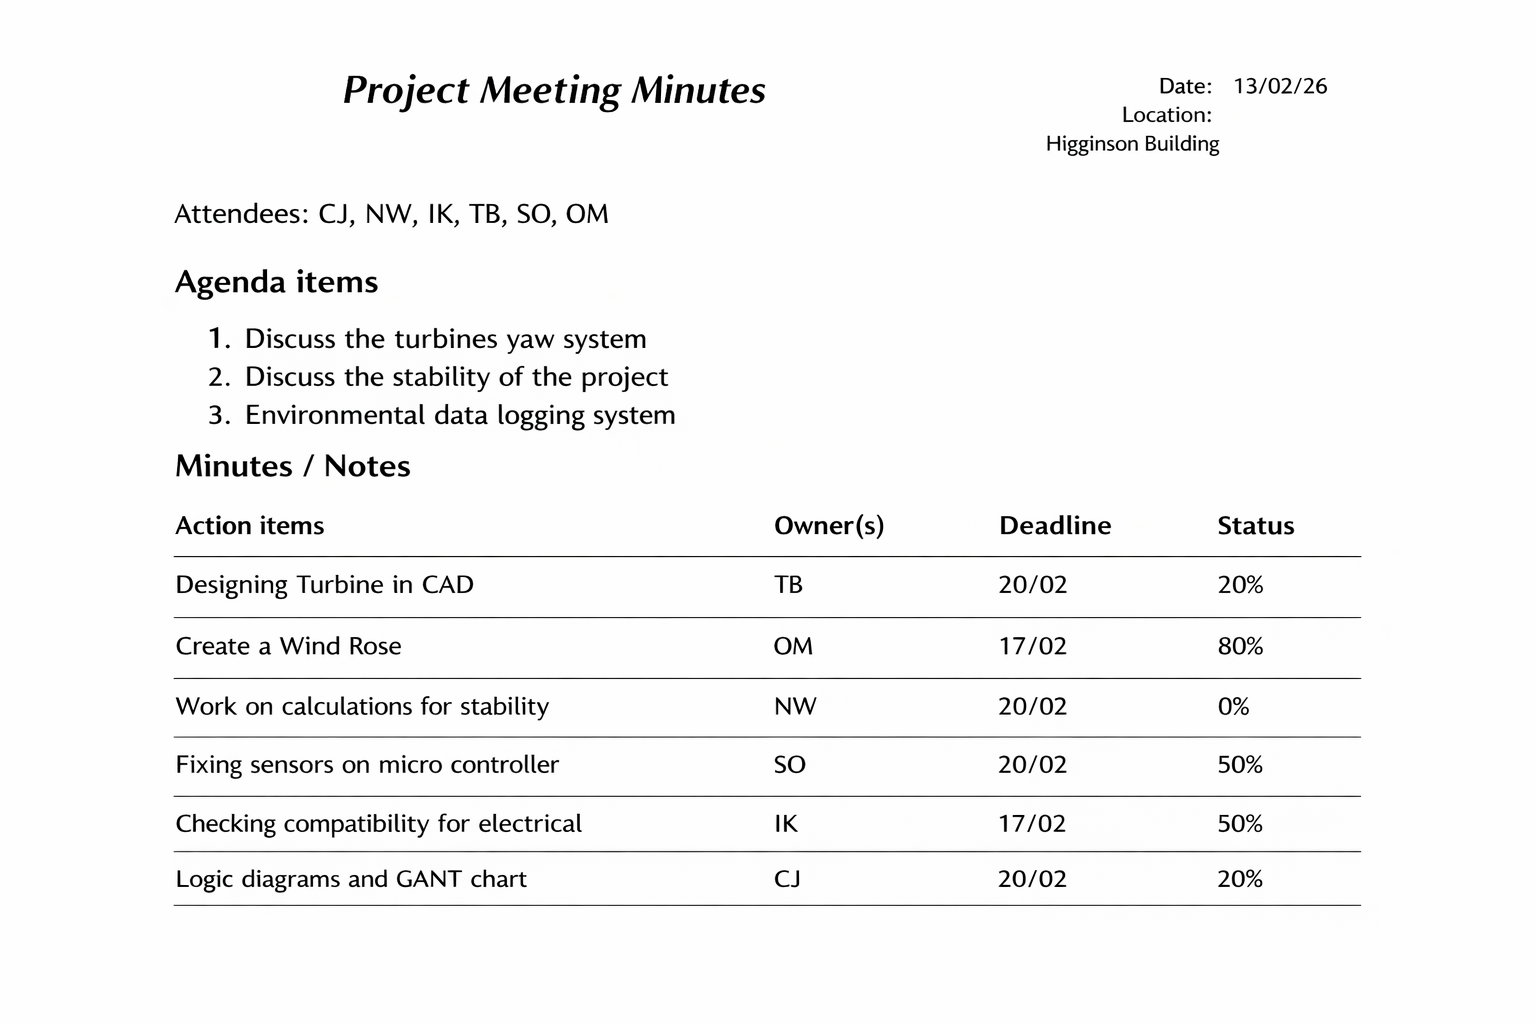
\includegraphics[width=1.1\textwidth, trim=3cm 3cm 0cm 1cm, clip]{figures/meetingminutes.png}
    \caption*{}
    \label{fig:meetingminutes}
\end{figure}

\vspace{10cm}

\section{Term 1 Gantt Chart}
\begin{figure}[h]
    \centering
    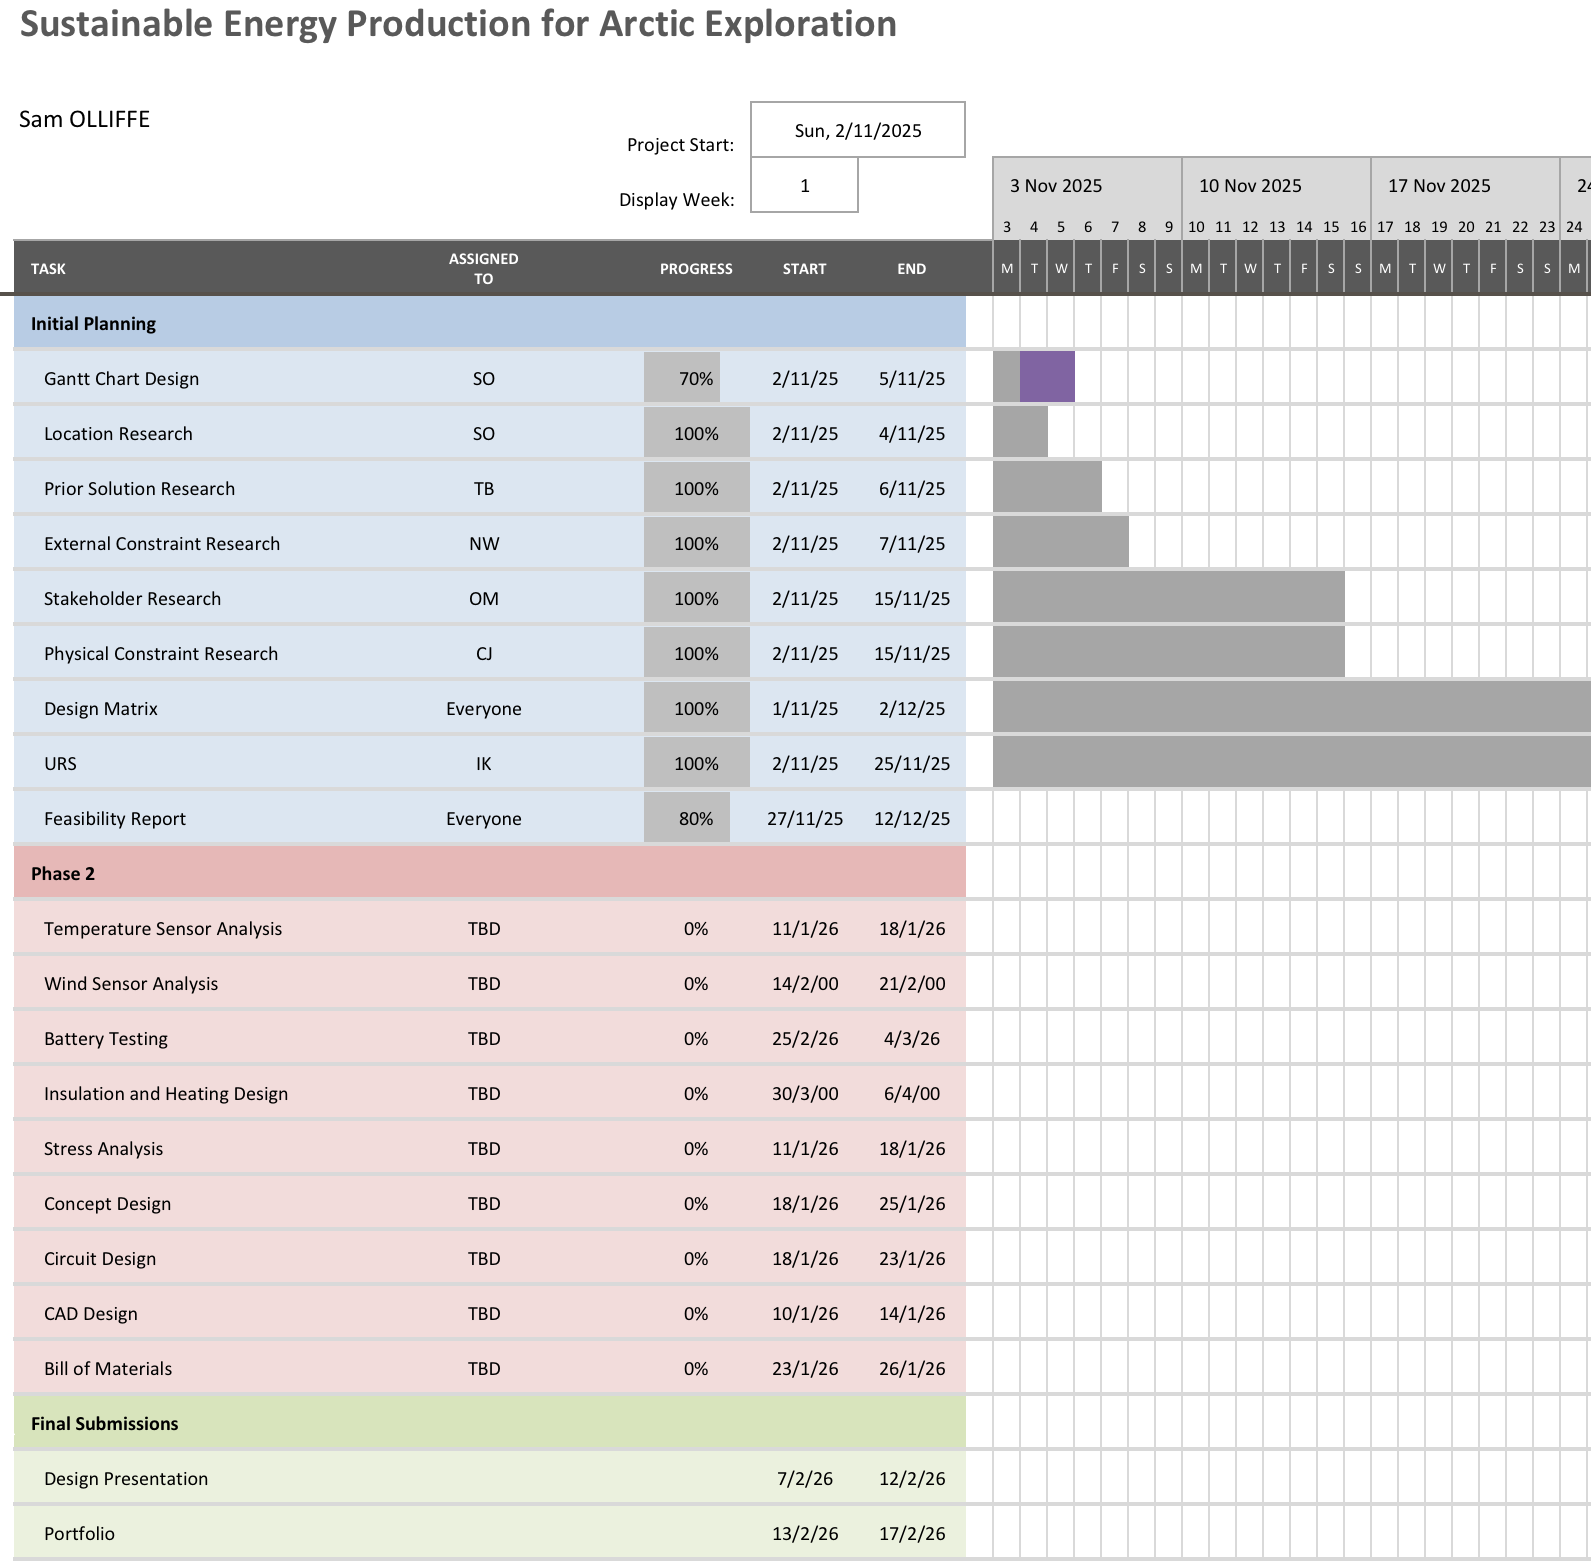
\includegraphics[width=1.1\textwidth]{figures/Project Schedule 10th Dec.png}
    \caption*{}
    \label{fig:meetingminutes}
\end{figure}
\end{document}